\section{Further invstigation of the Second Run~\label{sec:u_s_time_hist}} 
This section exhibits user and system time histograms on the second run of 
INC with its task length increasing from 1 second to 4096 seconds, via SEDONA. 
The detailed description of the base data is from Table~\ref{tab:exp_notes2}.

\subsection{User Time}

\begin{figure}[hp!]
	\centering
	\subfigure[User time frequency on INC1]{
		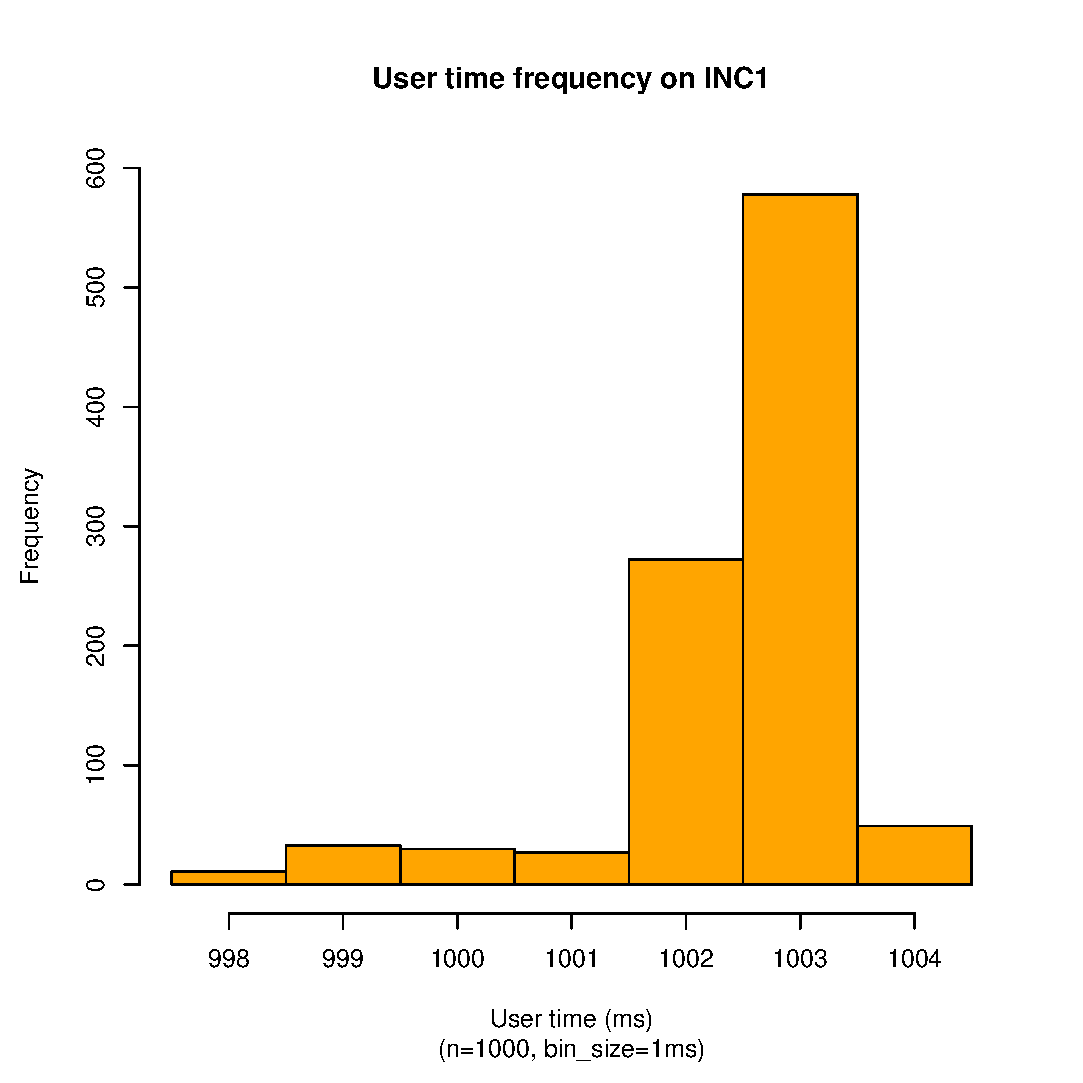
\includegraphics[scale=0.43]{u_s_time/1_sec_ut_hist.eps}
		\label{fig:inc1_ut_hist}
	}
	\subfigure[User time frequency on INC2]{
		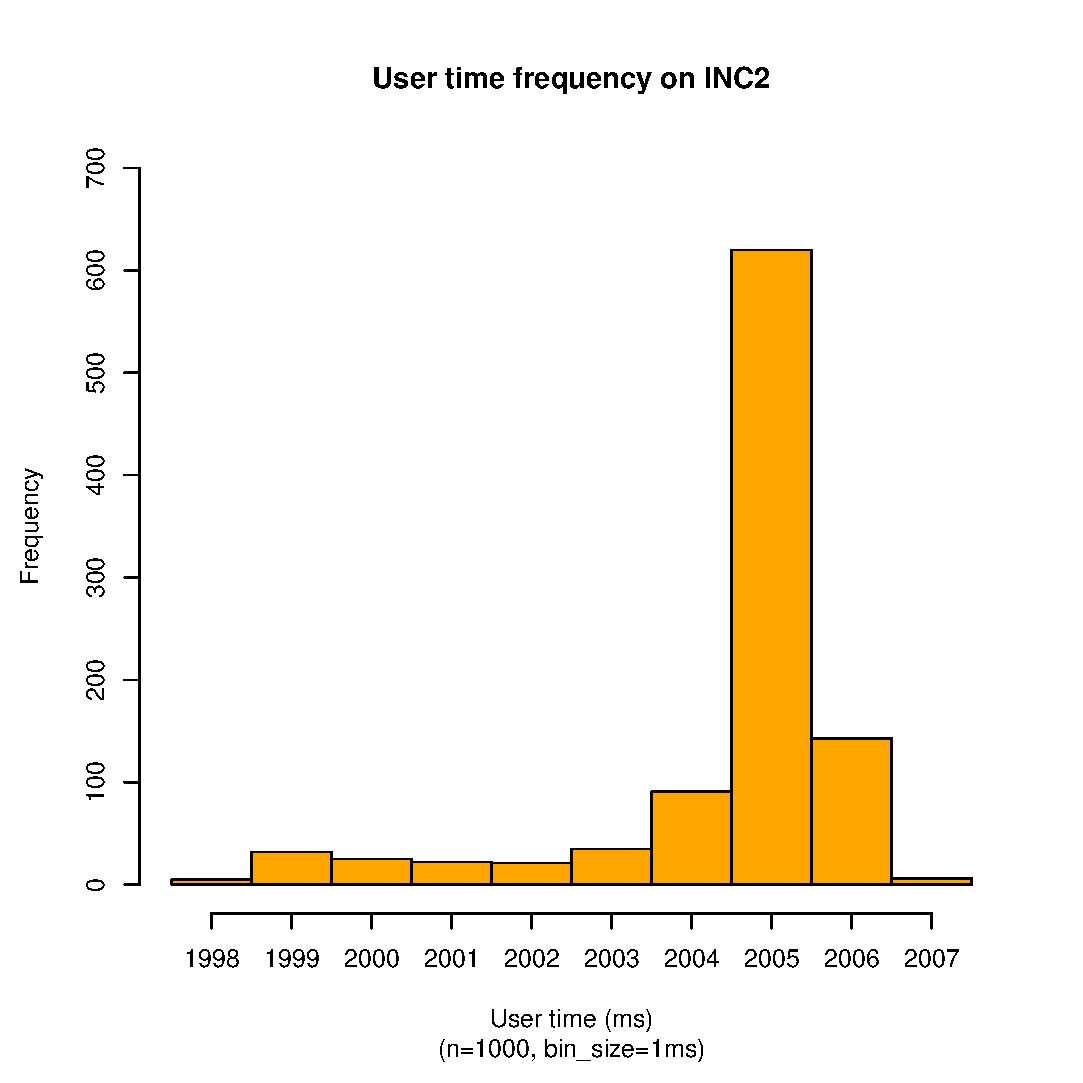
\includegraphics[scale=0.43]{u_s_time/2_sec_ut_hist.eps}
		\label{fig:inc2_ut_hist}
	}
	\subfigure[User time frequency on INC4]{
		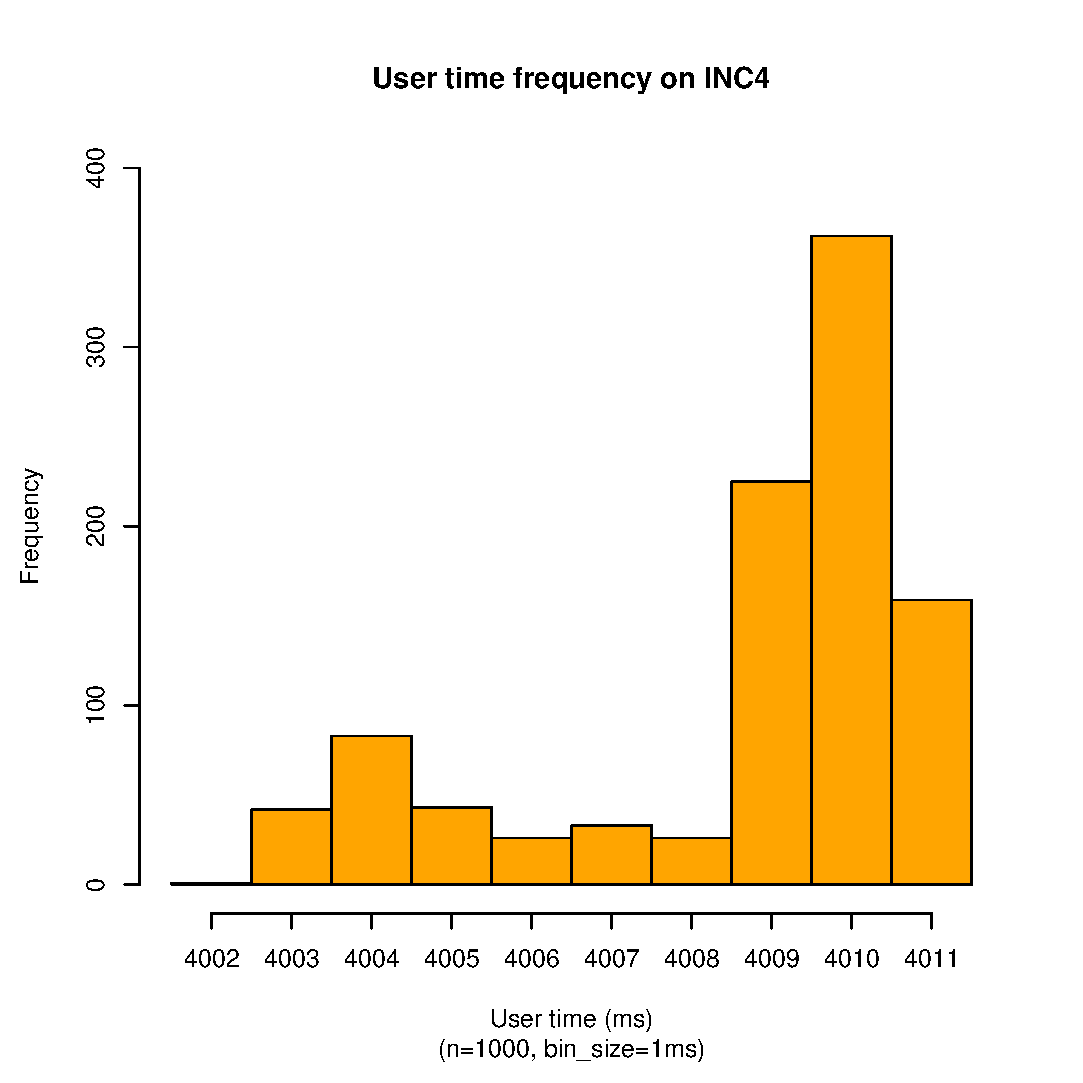
\includegraphics[scale=0.43]{u_s_time/4_sec_ut_hist.eps}
		\label{fig:inc4_ut_hist}
	}
	\subfigure[User time frequency on INC8]{
		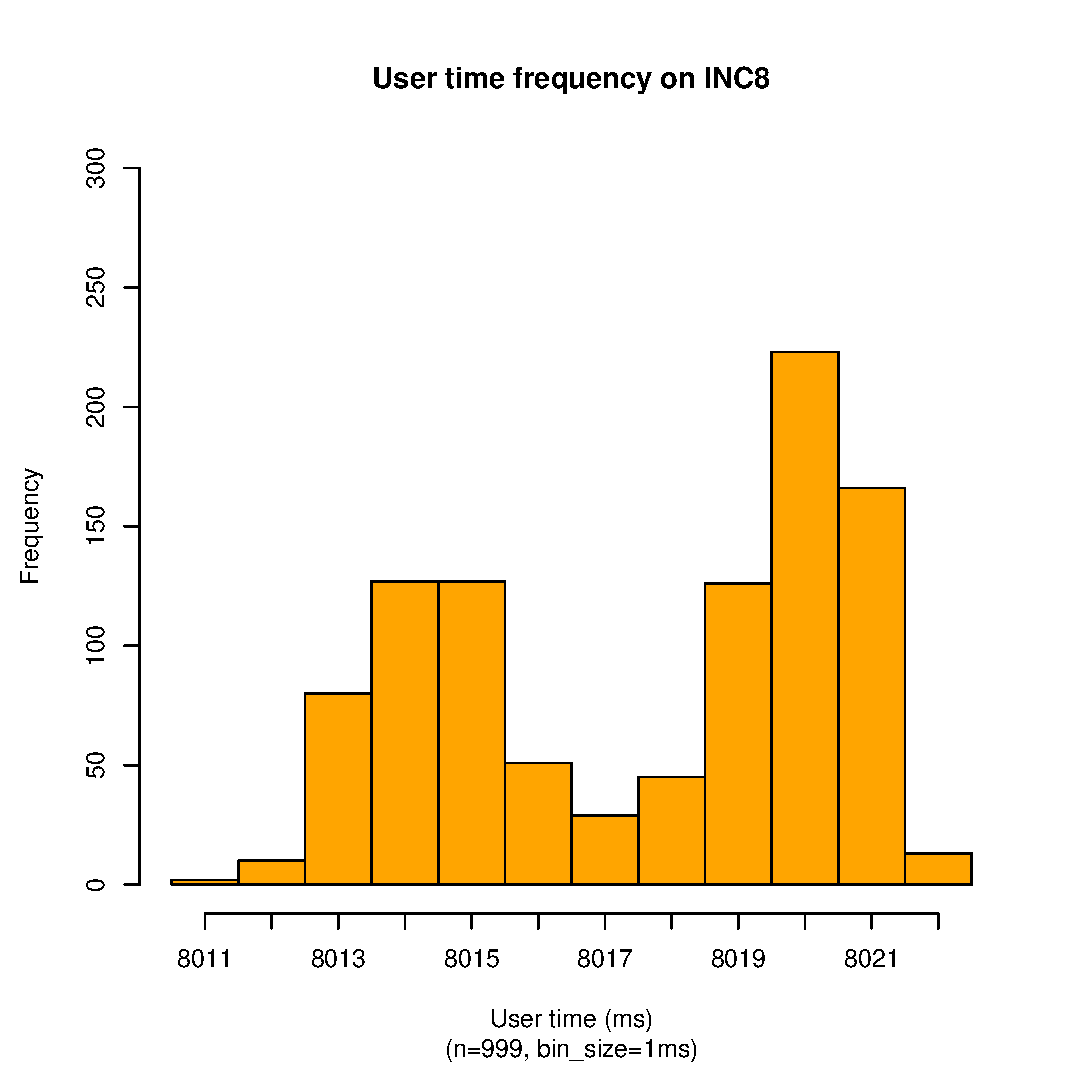
\includegraphics[scale=0.43]{u_s_time/8_sec_ut_hist.eps}
		\label{fig:inc8_ut_hist}
	}
	\caption{User Time Histograms of INC1 ... INC8~\label{fig:ut_hist1}}
\end{figure}

\begin{figure}[hp!]
	\centering
	\subfigure[User time frequency on INC16]{
		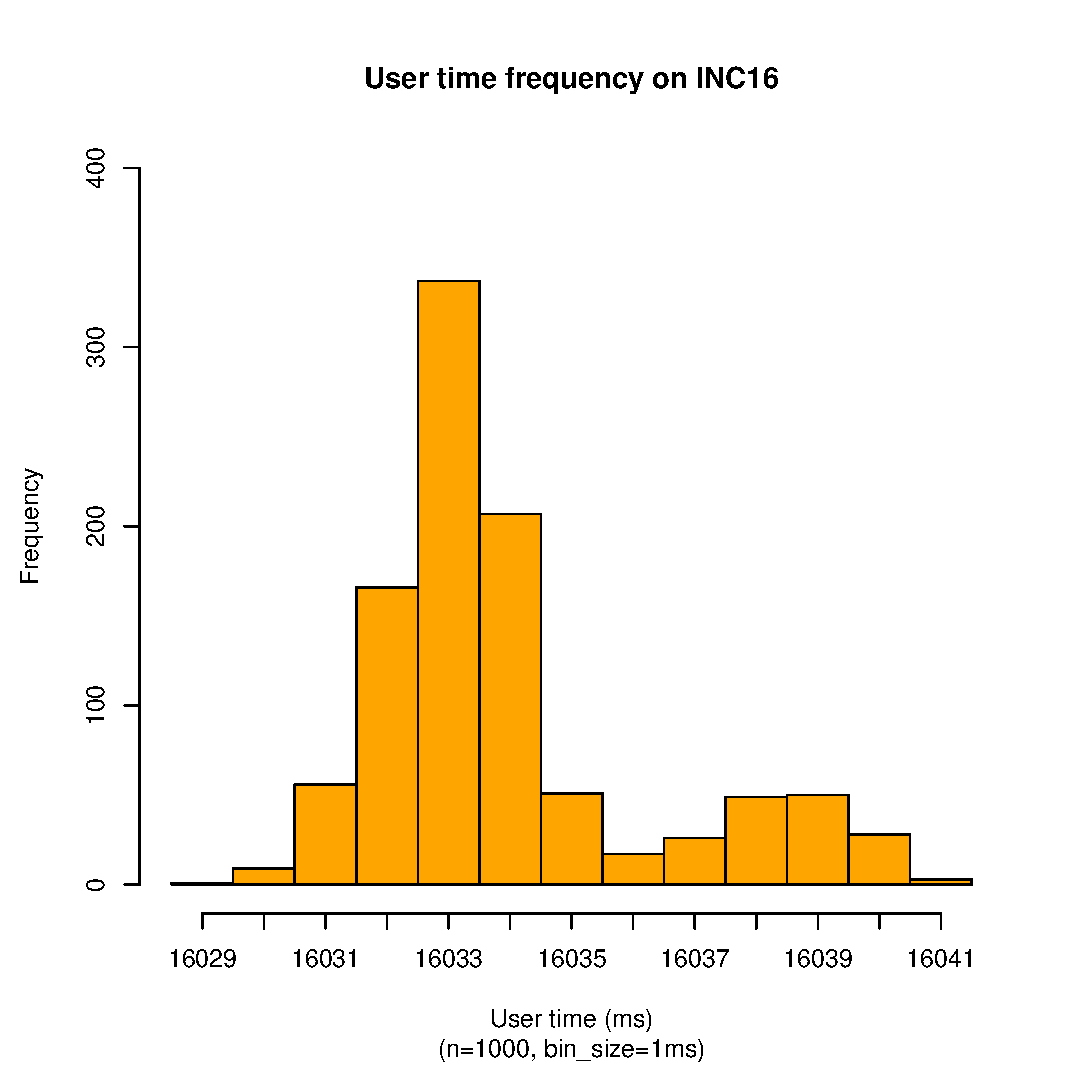
\includegraphics[scale=0.43]{u_s_time/16_sec_ut_hist.eps}
		\label{fig:inc16_ut_hist}
	}
	\subfigure[User time frequency on INC32]{
		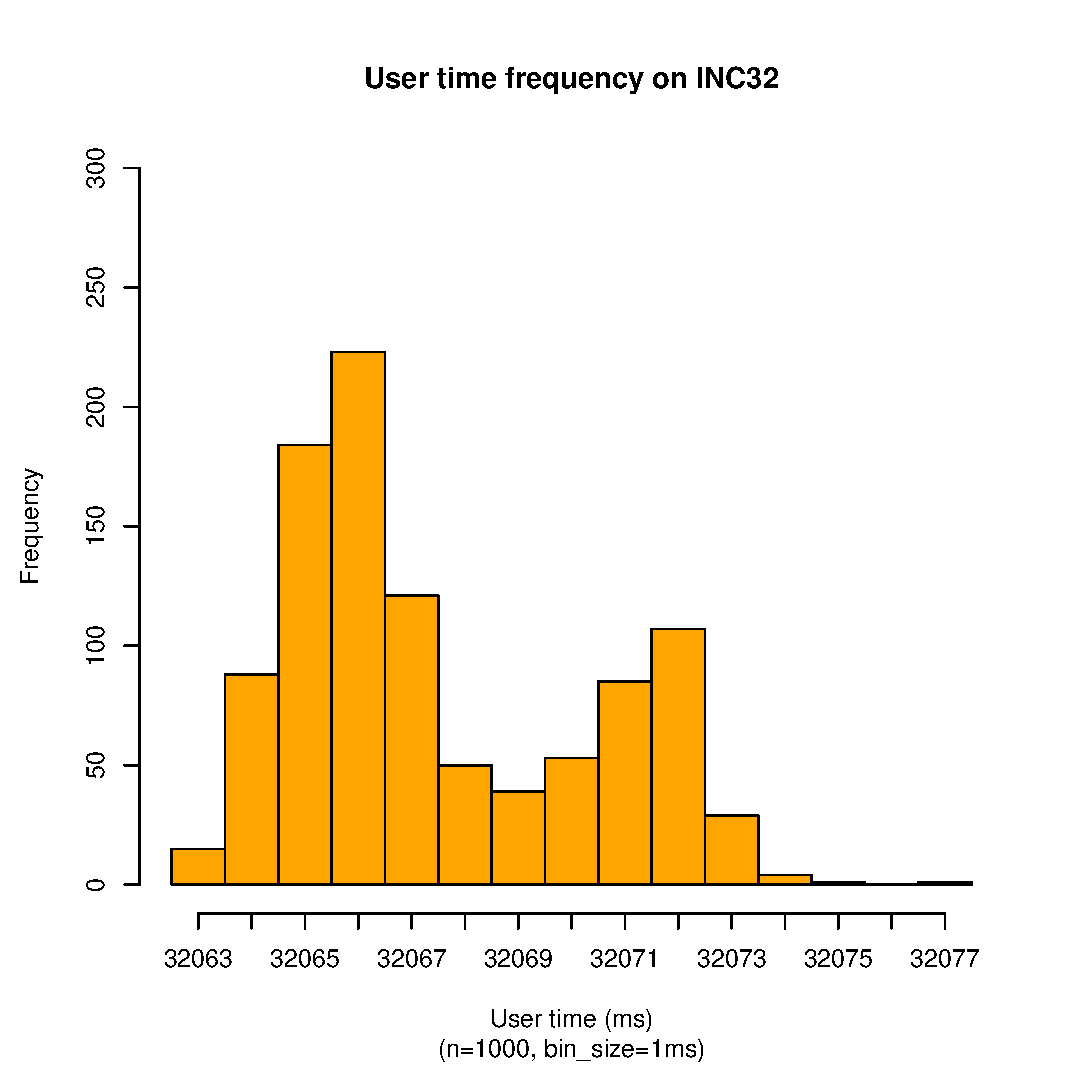
\includegraphics[scale=0.43]{u_s_time/32_sec_ut_hist.eps}
		\label{fig:inc32_ut_hist}
	}
	\subfigure[User time frequency on INC64]{
		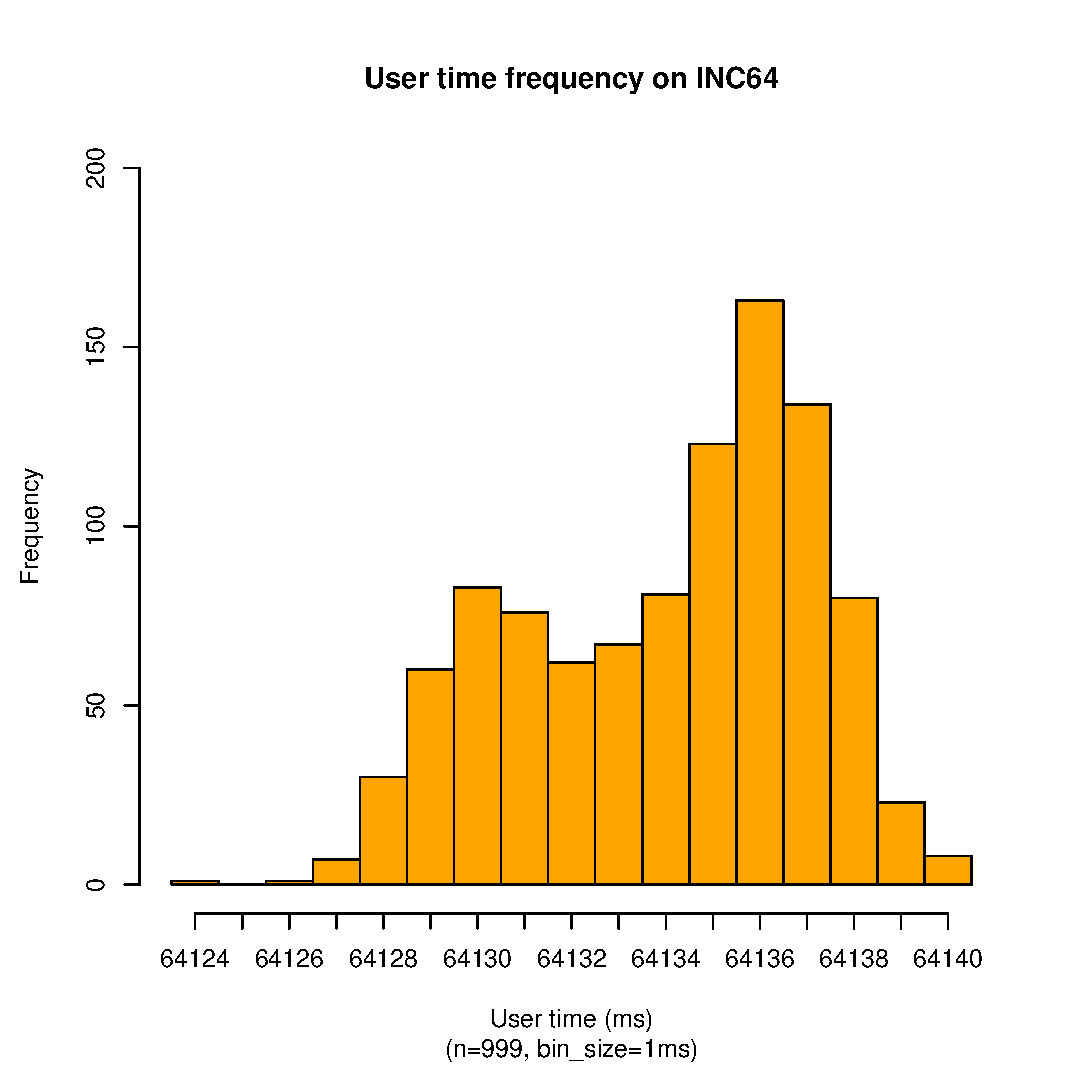
\includegraphics[scale=0.43]{u_s_time/64_sec_ut_hist.eps}
		\label{fig:inc64_ut_hist}
	}
	\caption{User Time Histograms of INC16 ... INC64~\label{fig:ut_hist2}}
\end{figure}

\begin{figure}[hp!]
	\centering
	\subfigure[User time frequency on INC96]{
		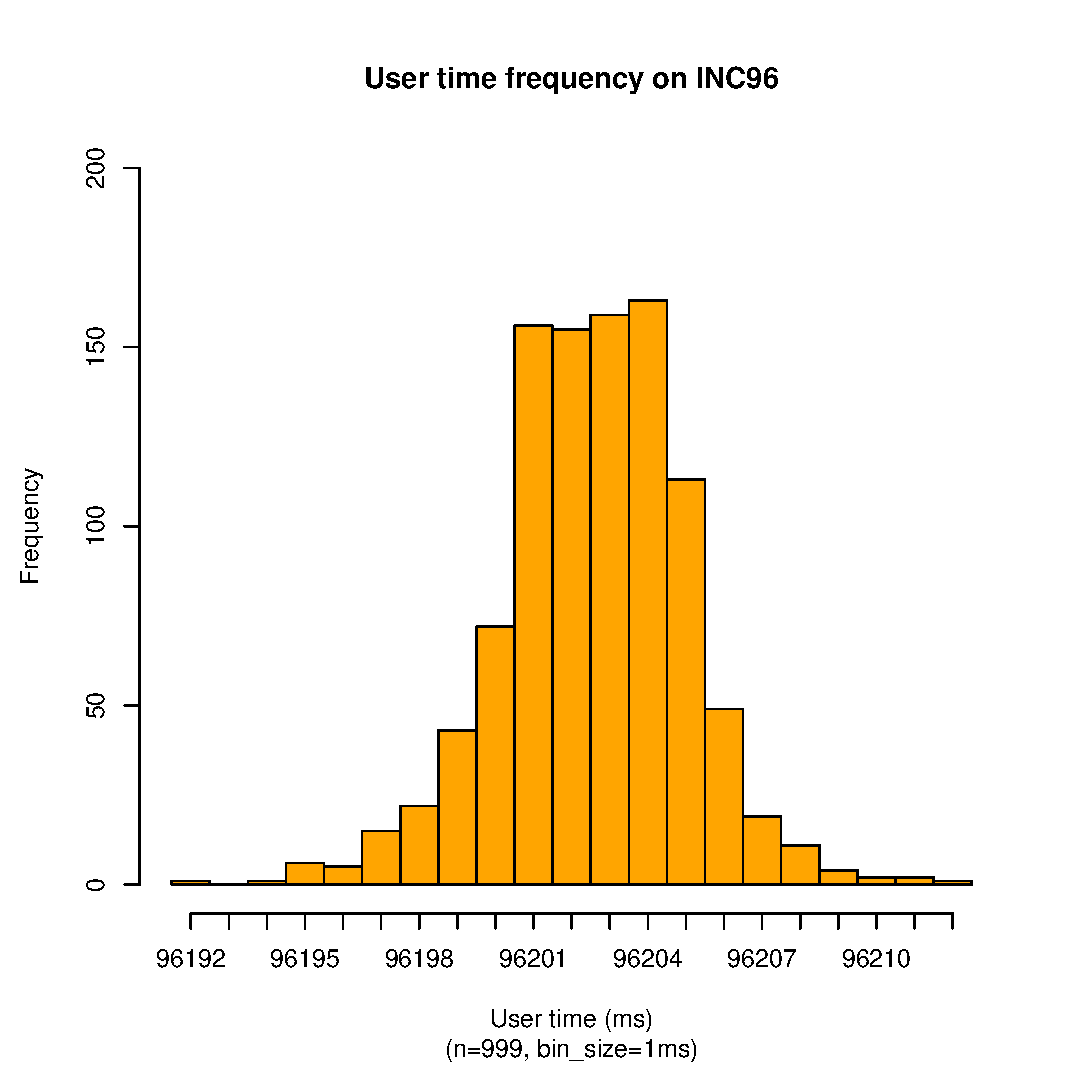
\includegraphics[scale=0.43]{u_s_time/96_sec_ut_hist.eps}
		\label{fig:inc96_ut_hist}
	}
	\subfigure[User time frequency on INC128]{
		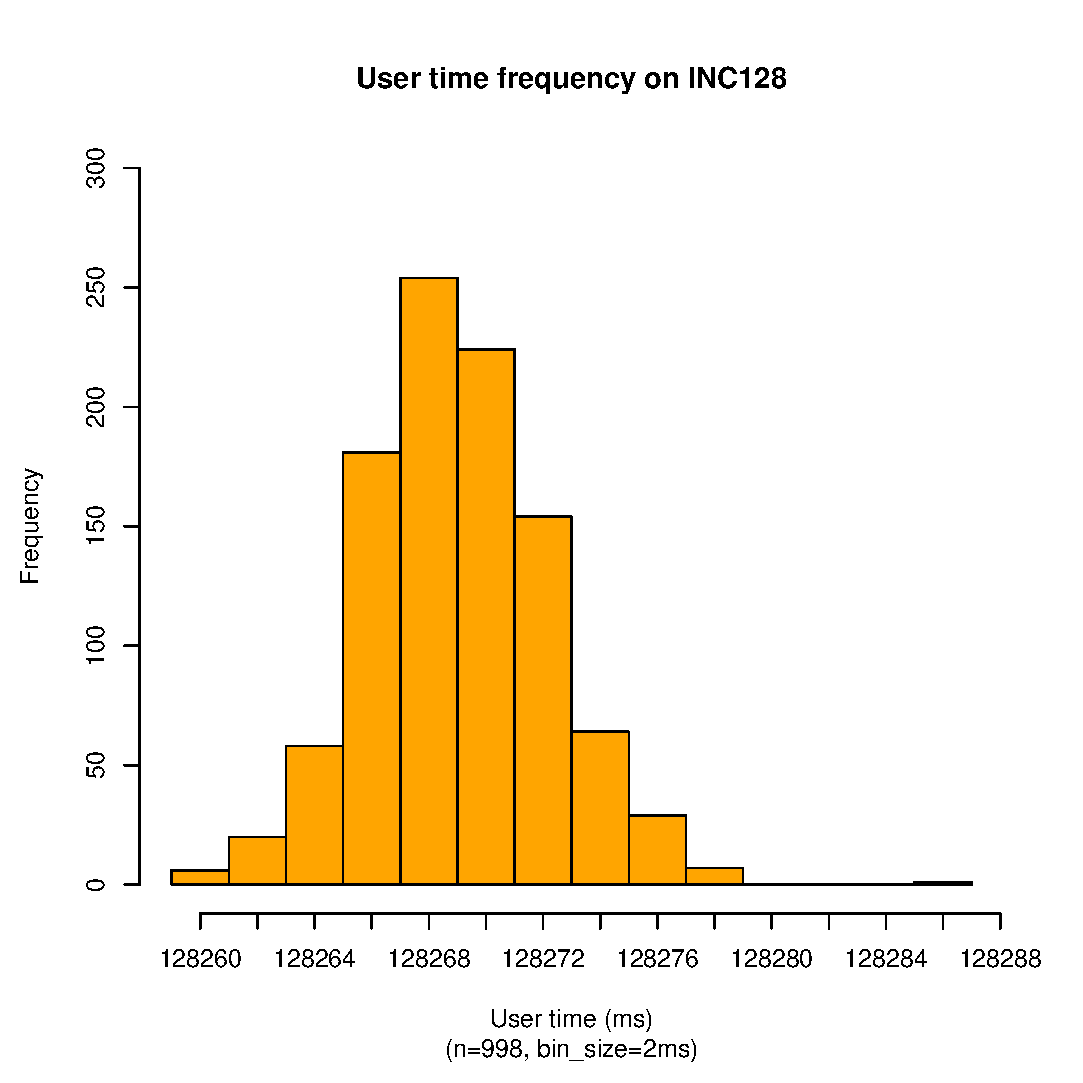
\includegraphics[scale=0.43]{u_s_time/128_sec_ut_hist2.eps}
		\label{fig:inc128_ut_hist2}
	}
	\subfigure[User time frequency on INC160]{
		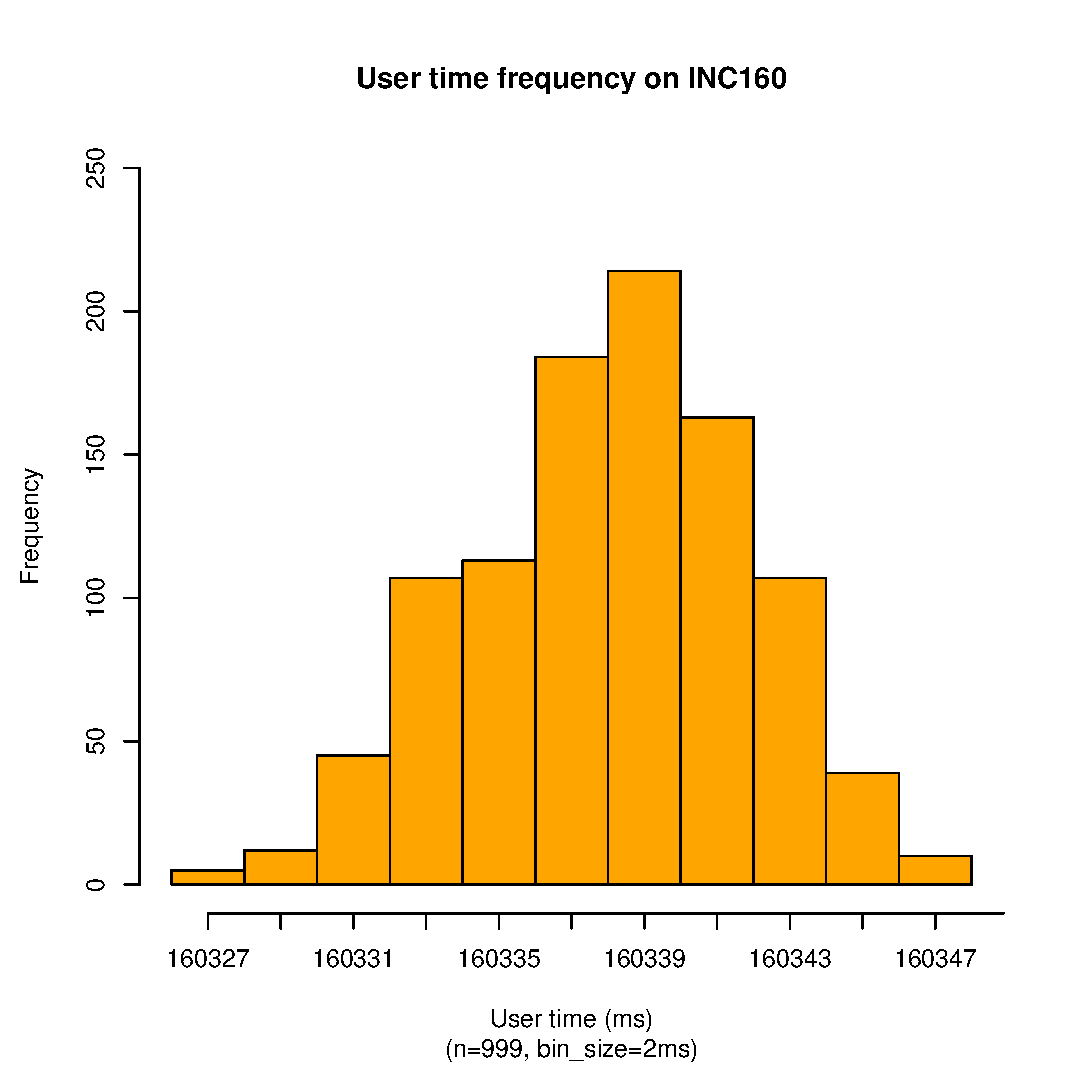
\includegraphics[scale=0.43]{u_s_time/160_sec_ut_hist.eps}
		\label{fig:inc160_ut_hist}
	}
	\subfigure[User time frequency on INC192]{
		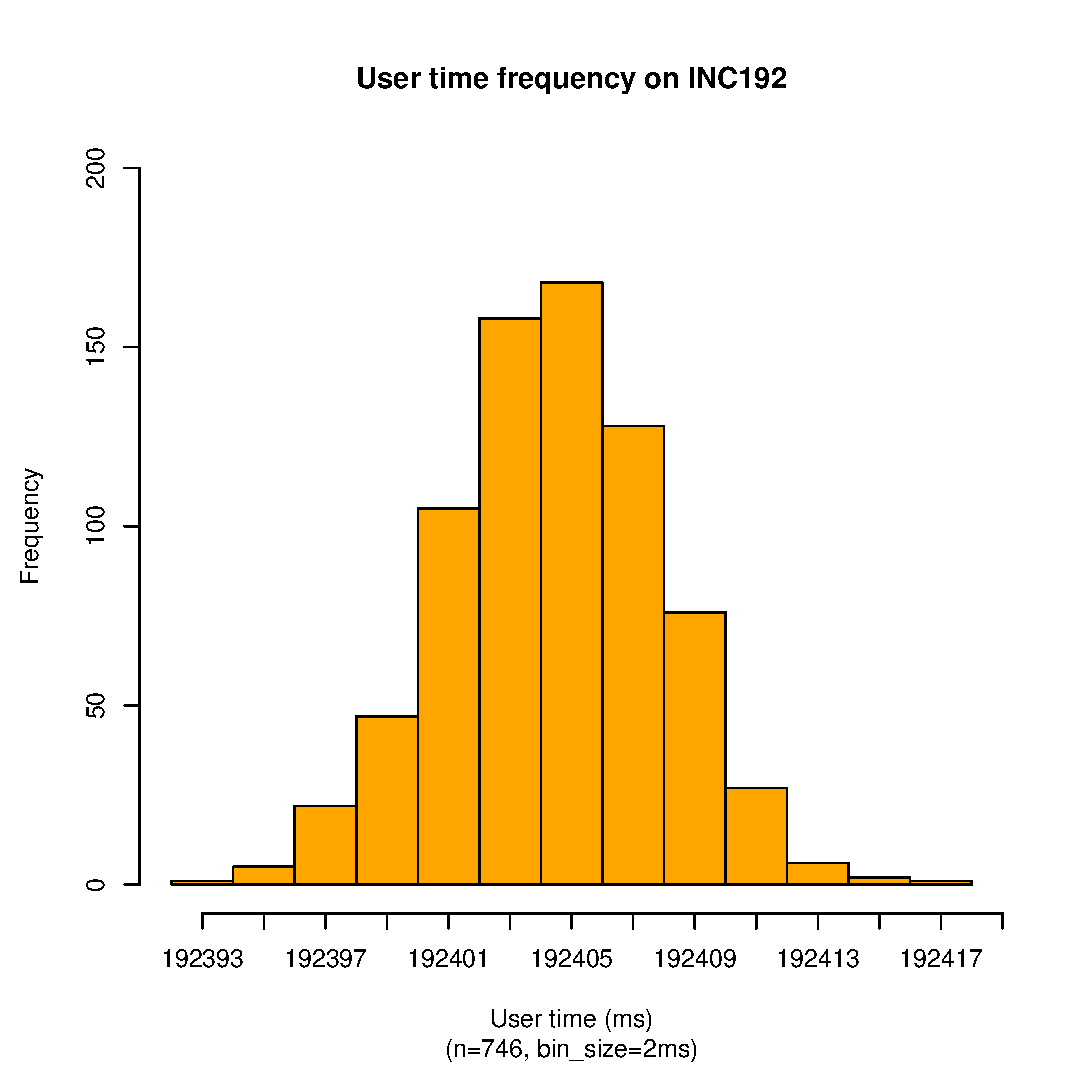
\includegraphics[scale=0.43]{u_s_time/192_sec_ut_hist.eps}
		\label{fig:inc192_ut_hist}
	}
	\caption{User Time Histograms of INC96 ... INC192~\label{fig:ut_hist3}}
\end{figure}

\begin{figure}[hp!]
	\centering
	\subfigure[User time frequency on INC256]{
		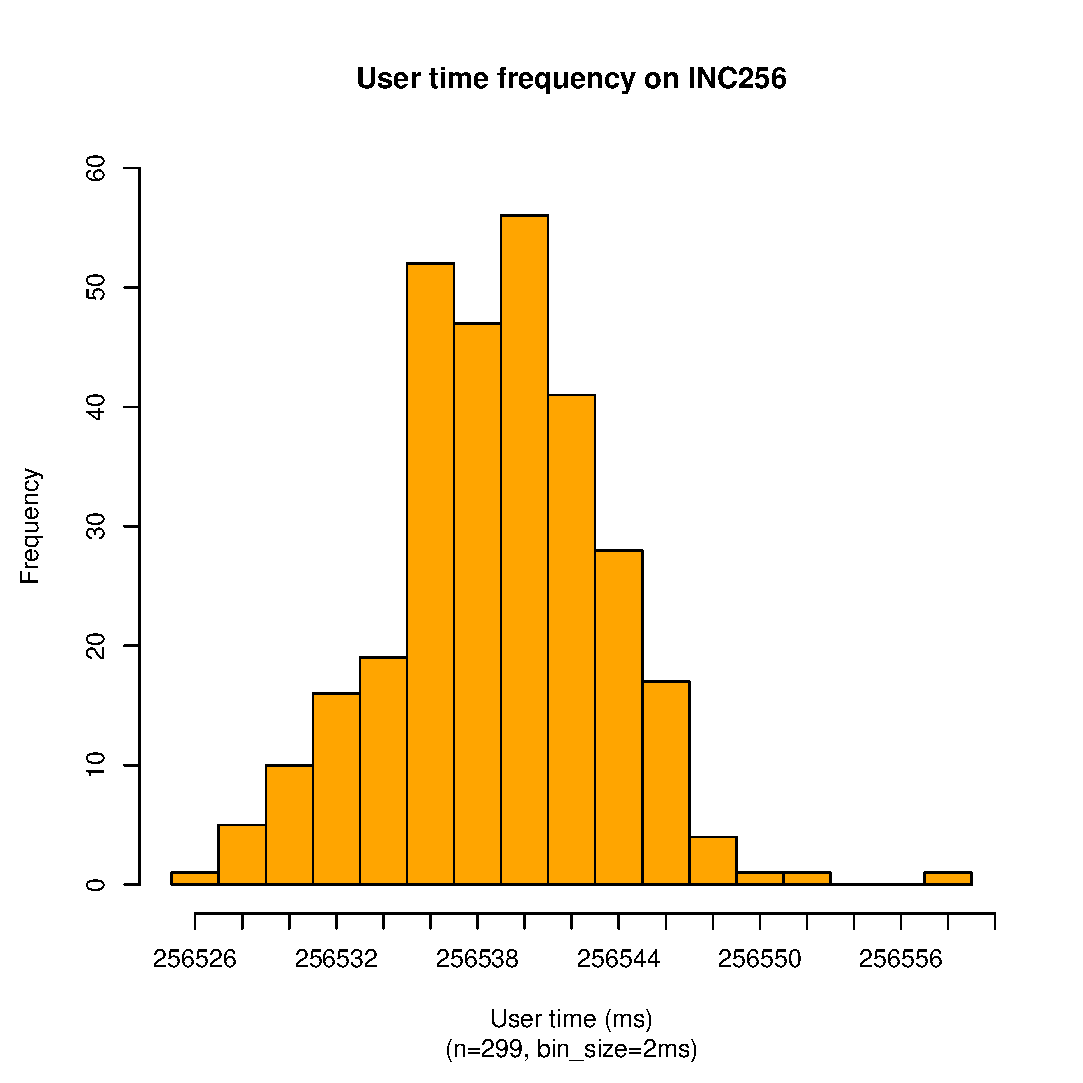
\includegraphics[scale=0.43]{u_s_time/256_sec_ut_hist.eps}
		\label{fig:inc256_ut_hist}
	}
	\subfigure[User time frequency on INC512 (with one extreme outlier of 513,259 msec removed)]{
		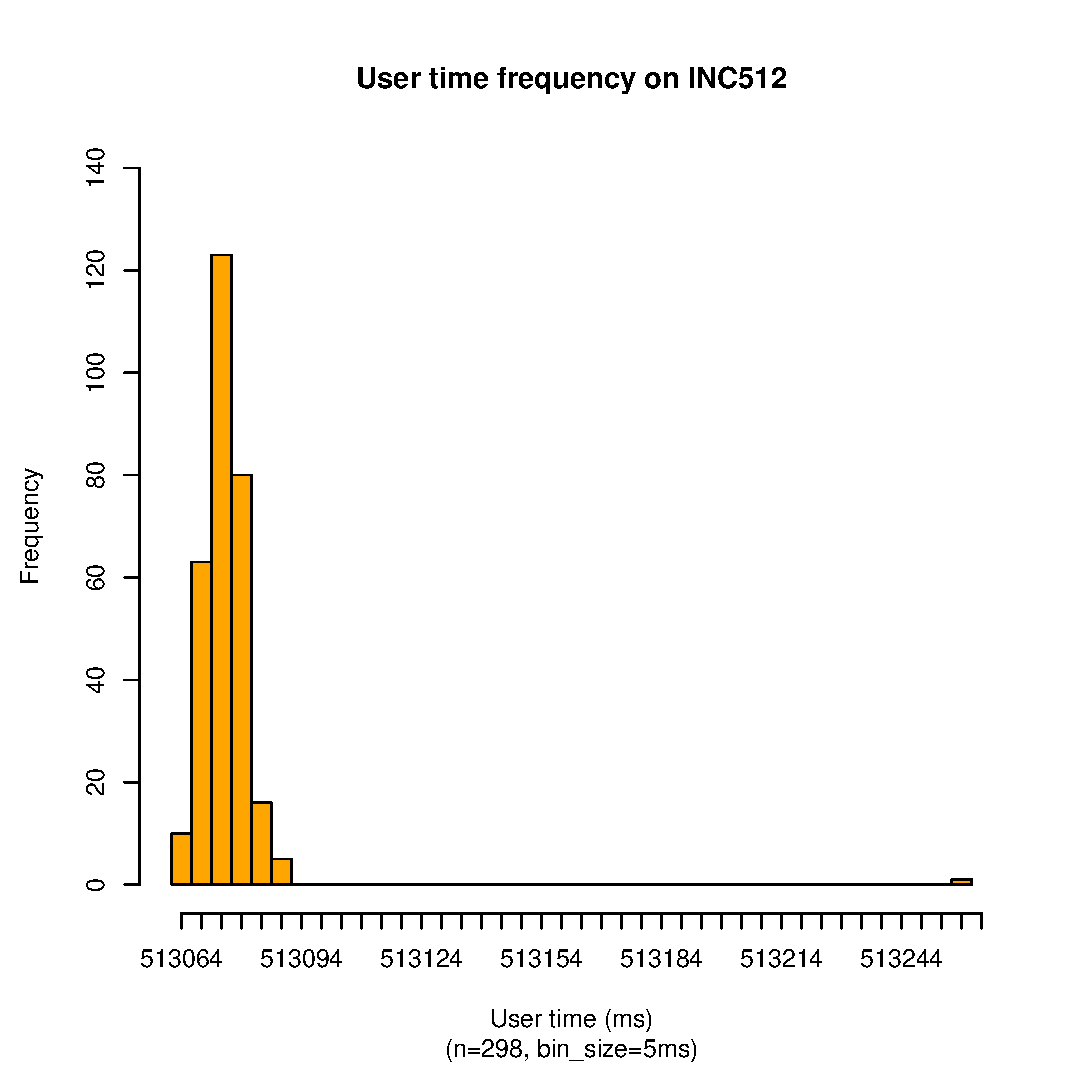
\includegraphics[scale=0.43]{u_s_time/512_sec_ut_hist.eps}
		\label{fig:inc512_ut_hist}
	}
	\subfigure[User time frequency on INC1024]{
		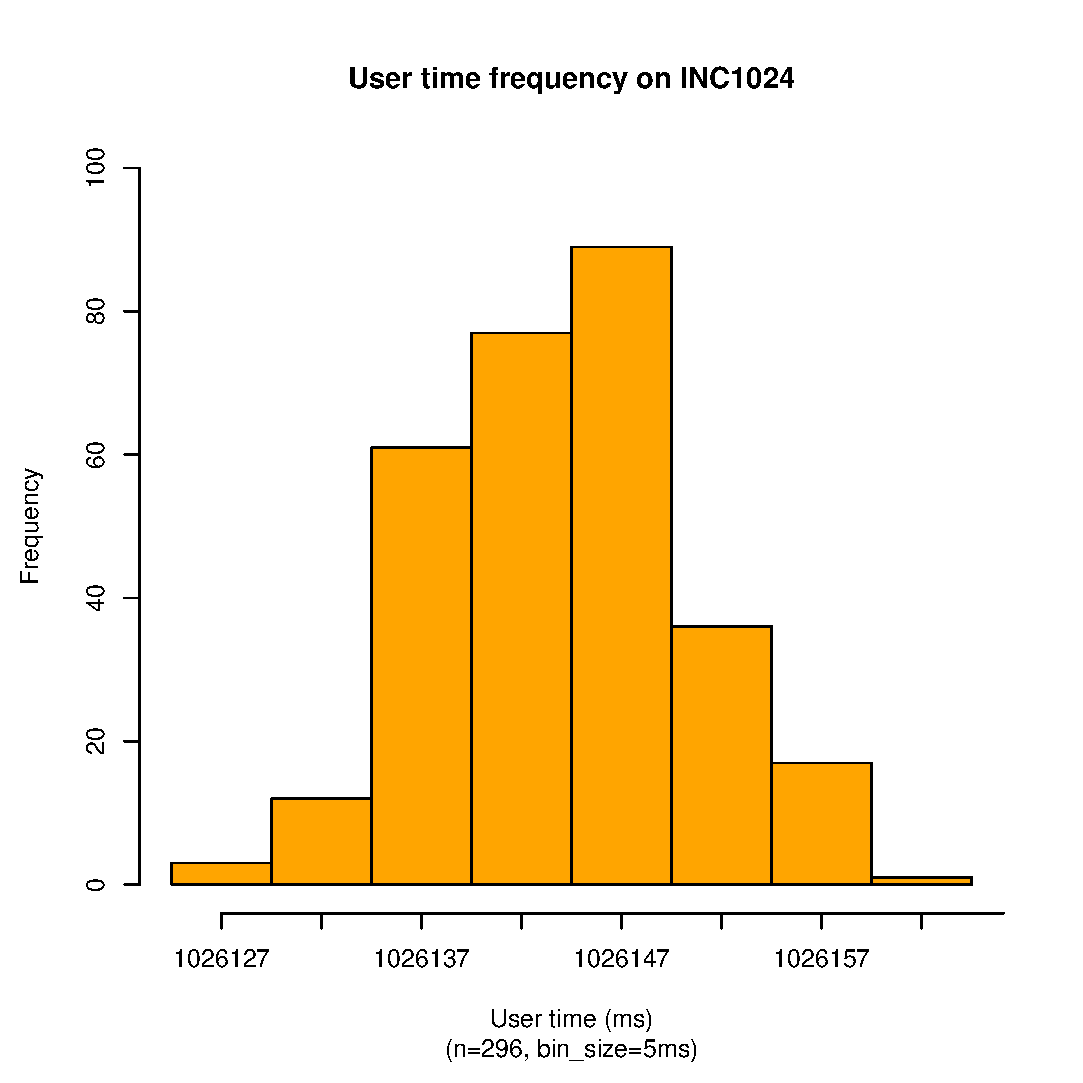
\includegraphics[scale=0.43]{u_s_time/1024_sec_ut_hist.eps}
		\label{fig:inc1024_ut_hist}
	}
	\caption{User Time Histograms of INC256 ... INC1024~\label{fig:ut_hist4}}
\end{figure}

%\begin{figure}[hp!]
%	\centering
%	\subfigure[User time frequency on INC2048]{
%		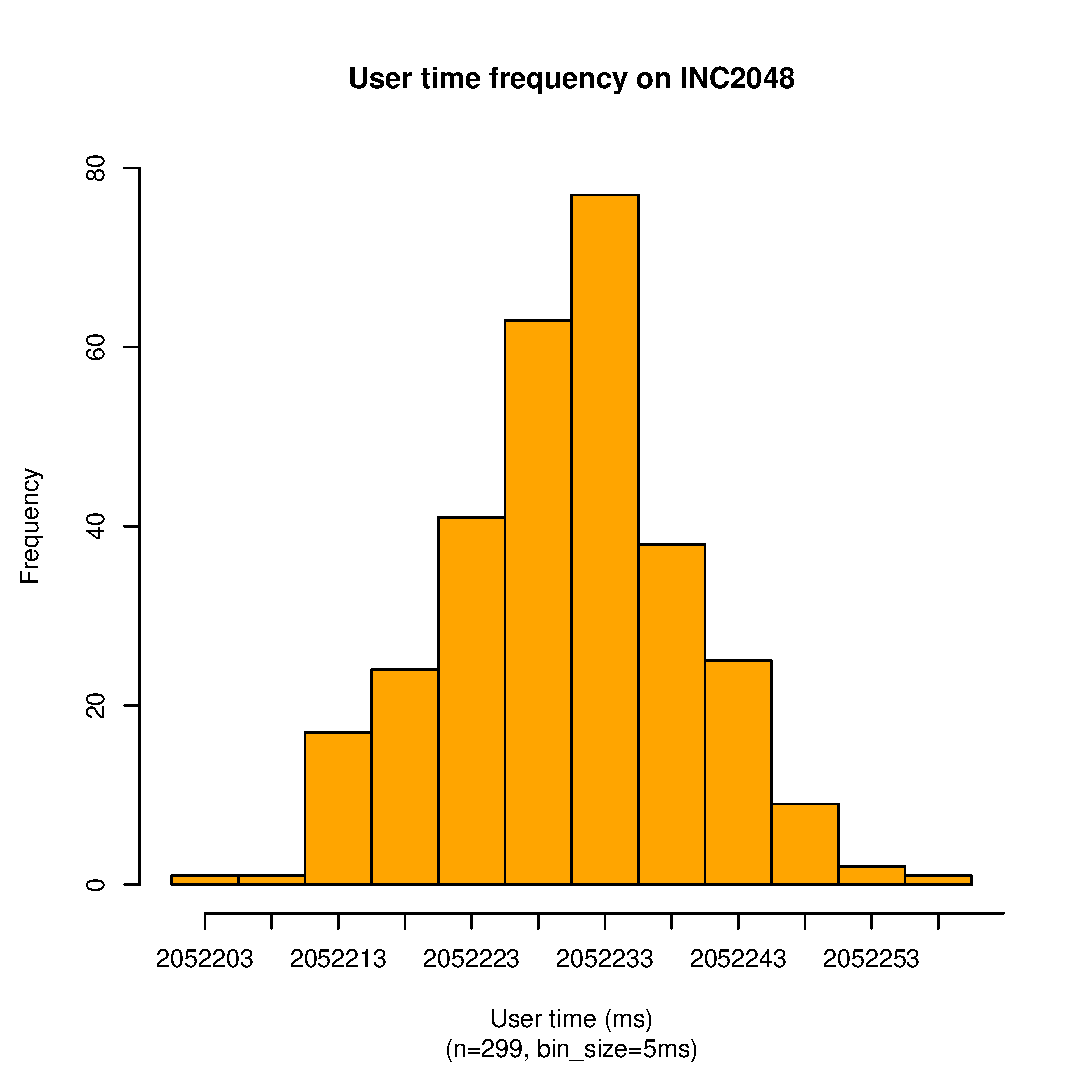
\includegraphics[scale=0.43]{u_s_time/2048_sec_ut_hist.eps}
%		\label{fig:inc2048_ut_hist}
%	}
%	\subfigure[User time frequency on INC4096]{
%		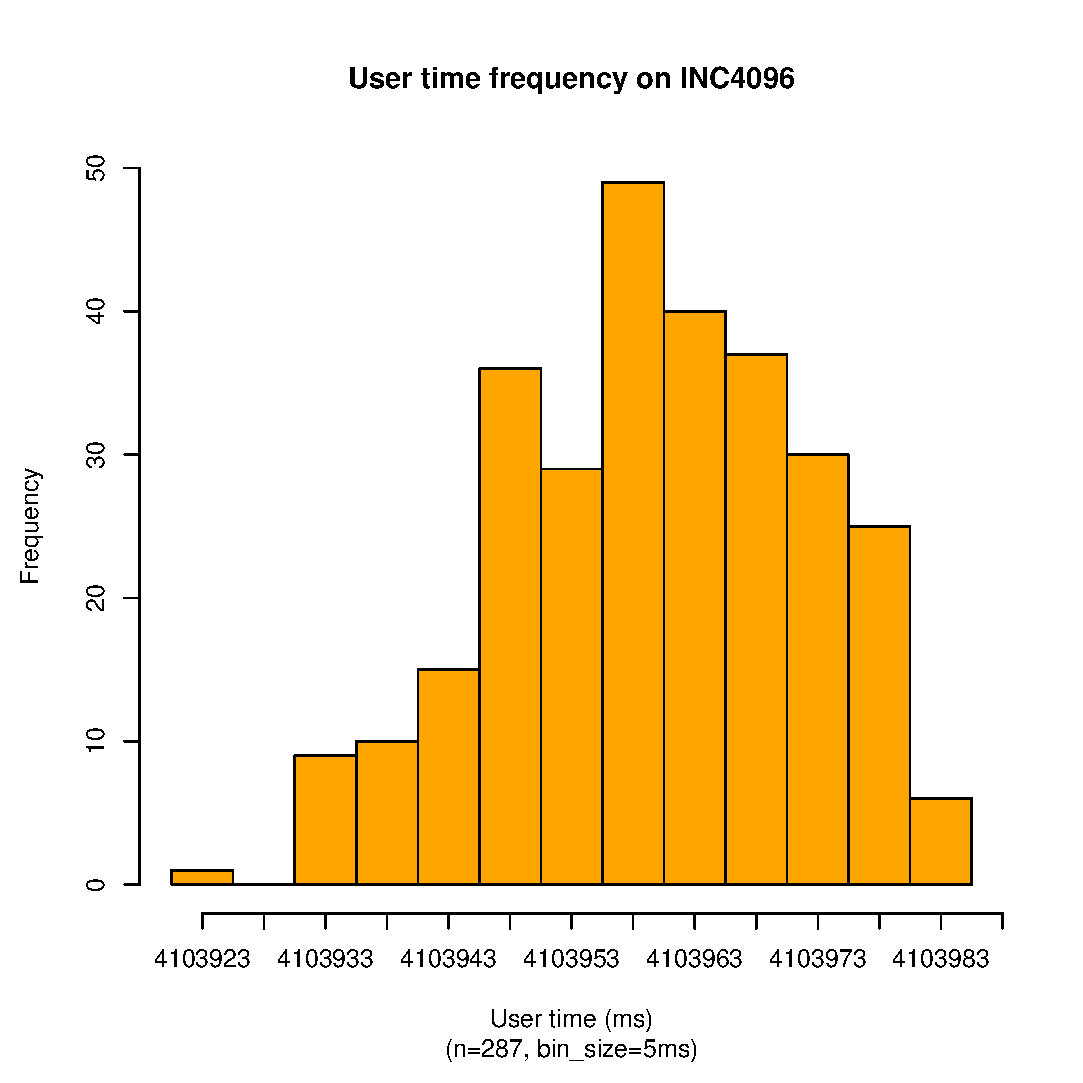
\includegraphics[scale=0.43]{u_s_time/4096_sec_ut_hist.eps}
%		\label{fig:inc4096_ut_hist}
%	}
%	\caption{User Time Histograms of INC2048 and INC4096~\label{fig:ut_hist5}}
%\end{figure}

\vspace\fill
\clearpage

\subsection{System Time}

\begin{figure}[hp!]
	\centering
	\subfigure[System time frequency on INC1]{
		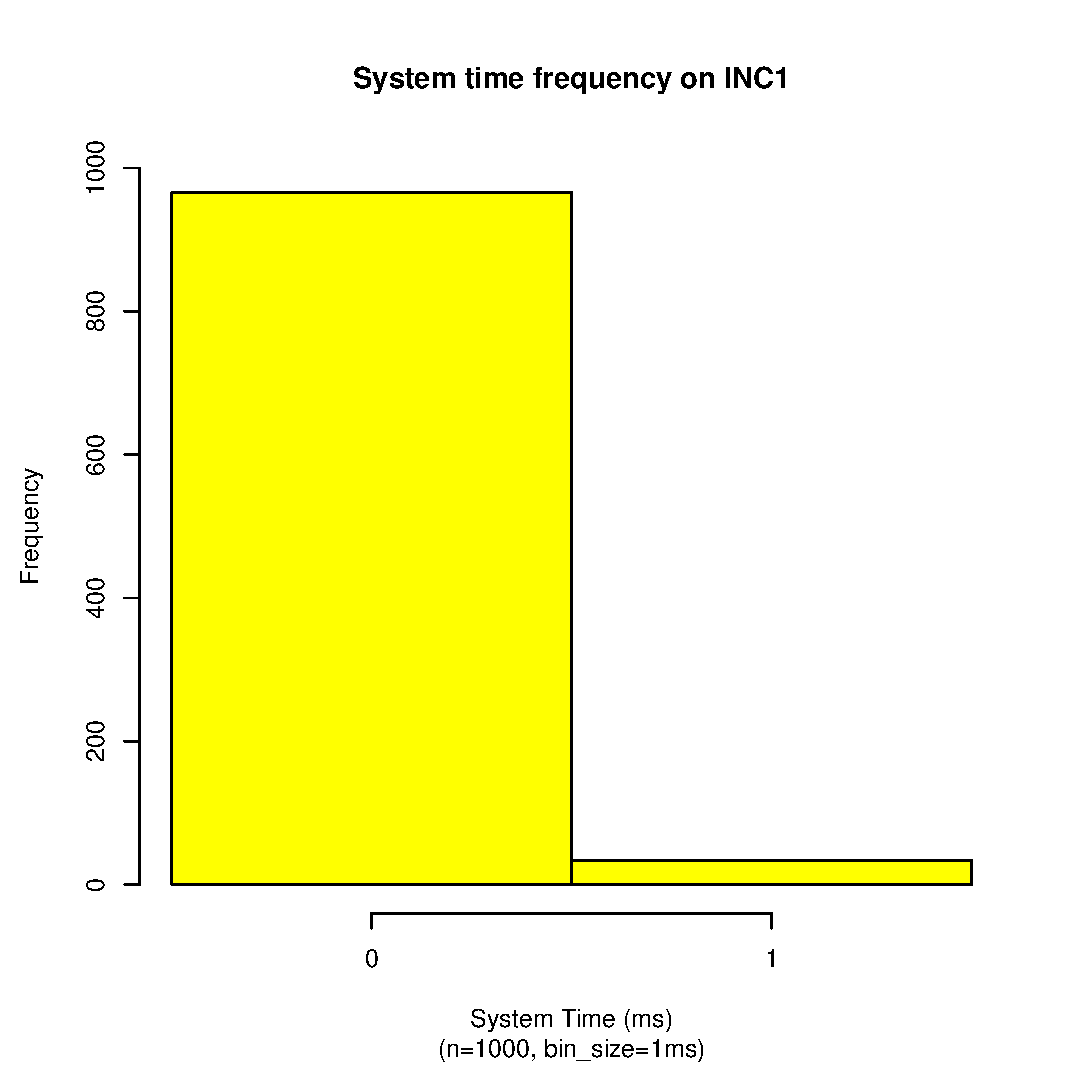
\includegraphics[scale=0.43]{u_s_time/1_sec_st_hist.eps}
		\label{fig:inc1_hist_v5}
	}
	\subfigure[System time frequency on INC2]{
		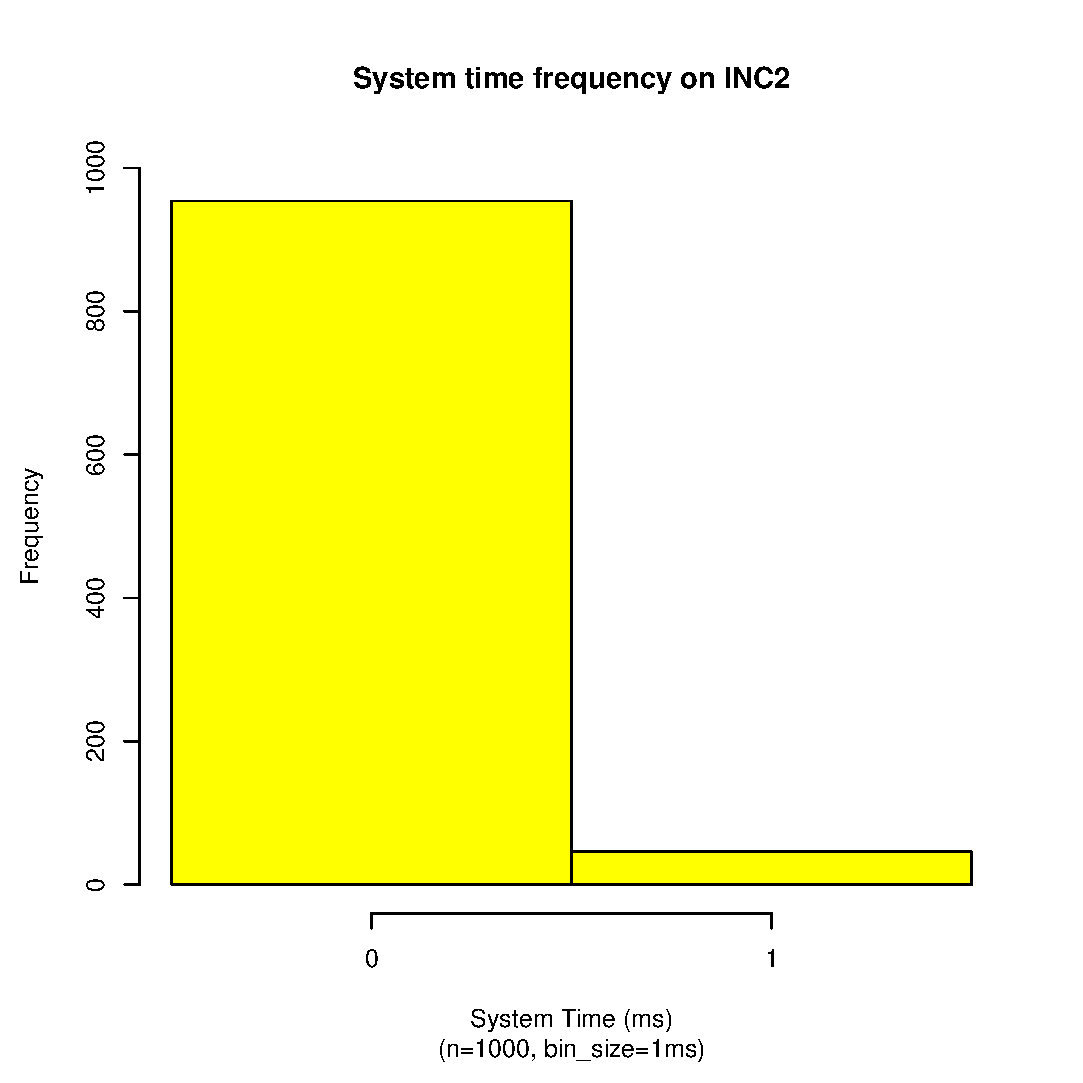
\includegraphics[scale=0.43]{u_s_time/2_sec_st_hist.eps}
		\label{fig:inc2_hist_st}
	}
	\subfigure[System time frequency on INC4]{
		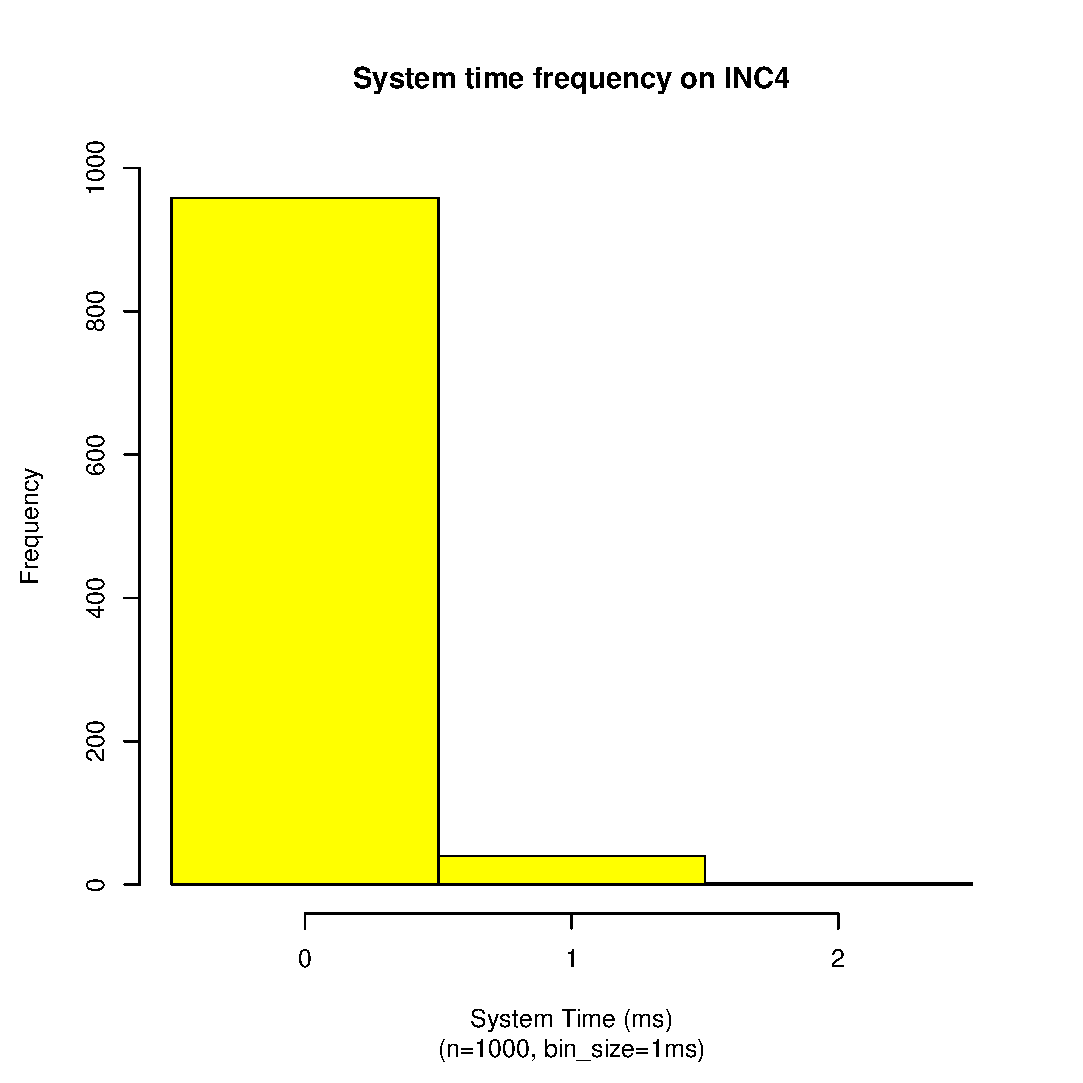
\includegraphics[scale=0.43]{u_s_time/4_sec_st_hist.eps}
		\label{fig:inc4_hist_st}
	}
	\subfigure[System time frequency on INC8]{
		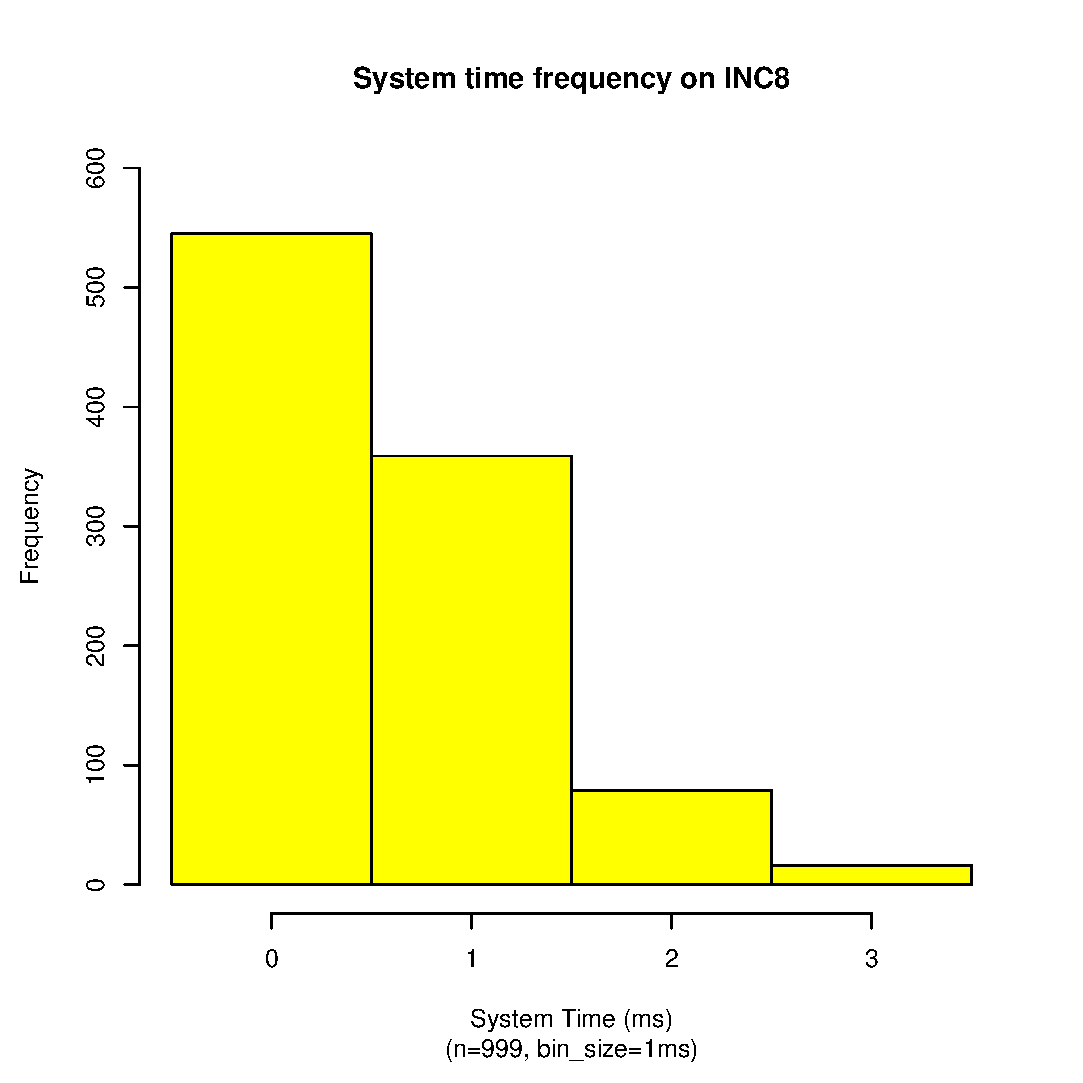
\includegraphics[scale=0.43]{u_s_time/8_sec_st_hist.eps}
		\label{fig:inc8_hist_st}
	}
	\caption{System Time Histograms of INC1 ... INC8~\label{fig:st_hist1}}
\end{figure}

\begin{figure}[hp!]
	\centering
	\subfigure[System time frequency on INC16]{
		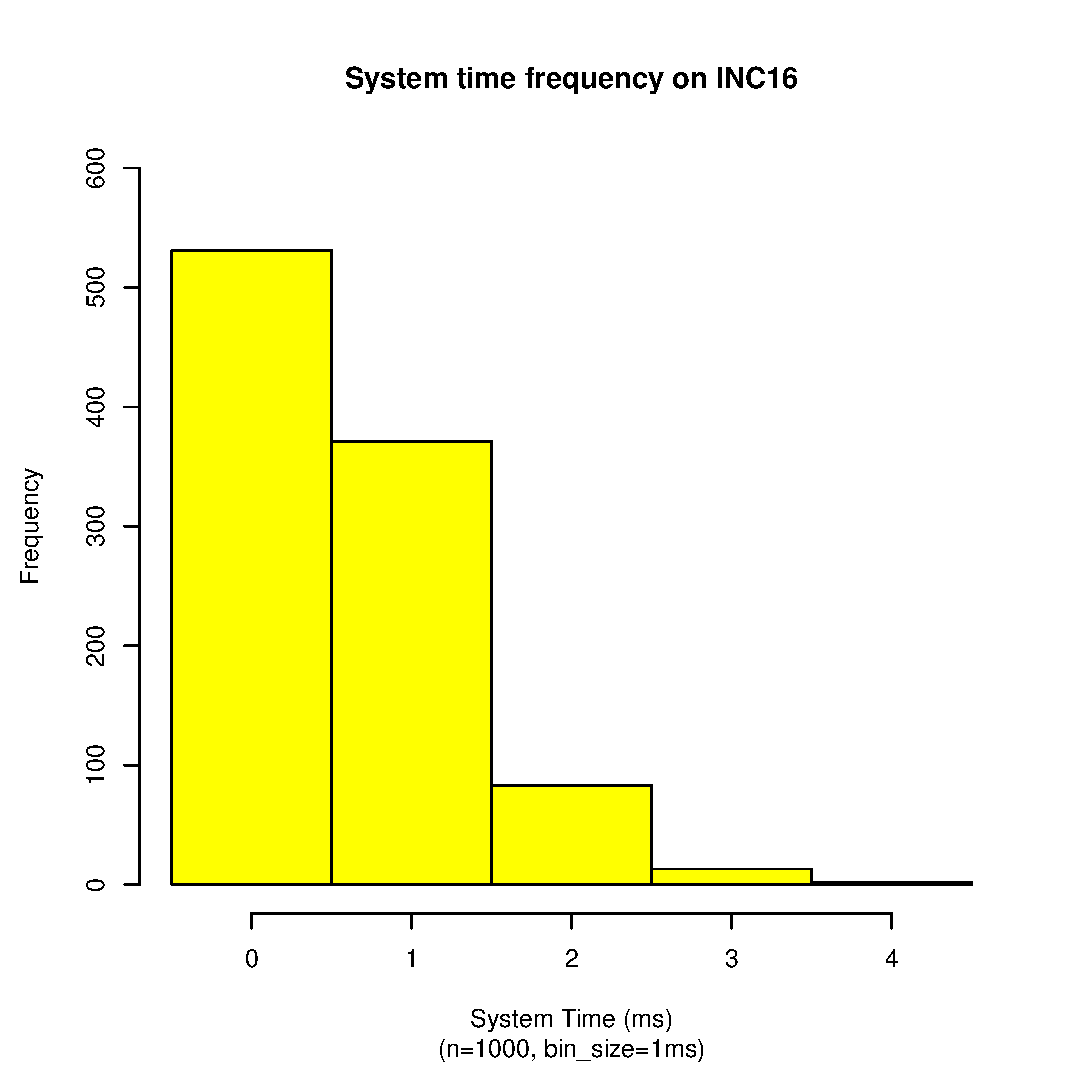
\includegraphics[scale=0.43]{u_s_time/16_sec_st_hist.eps}
		\label{fig:inc16_hist_st}
	}
	\subfigure[System time frequency on INC32]{
		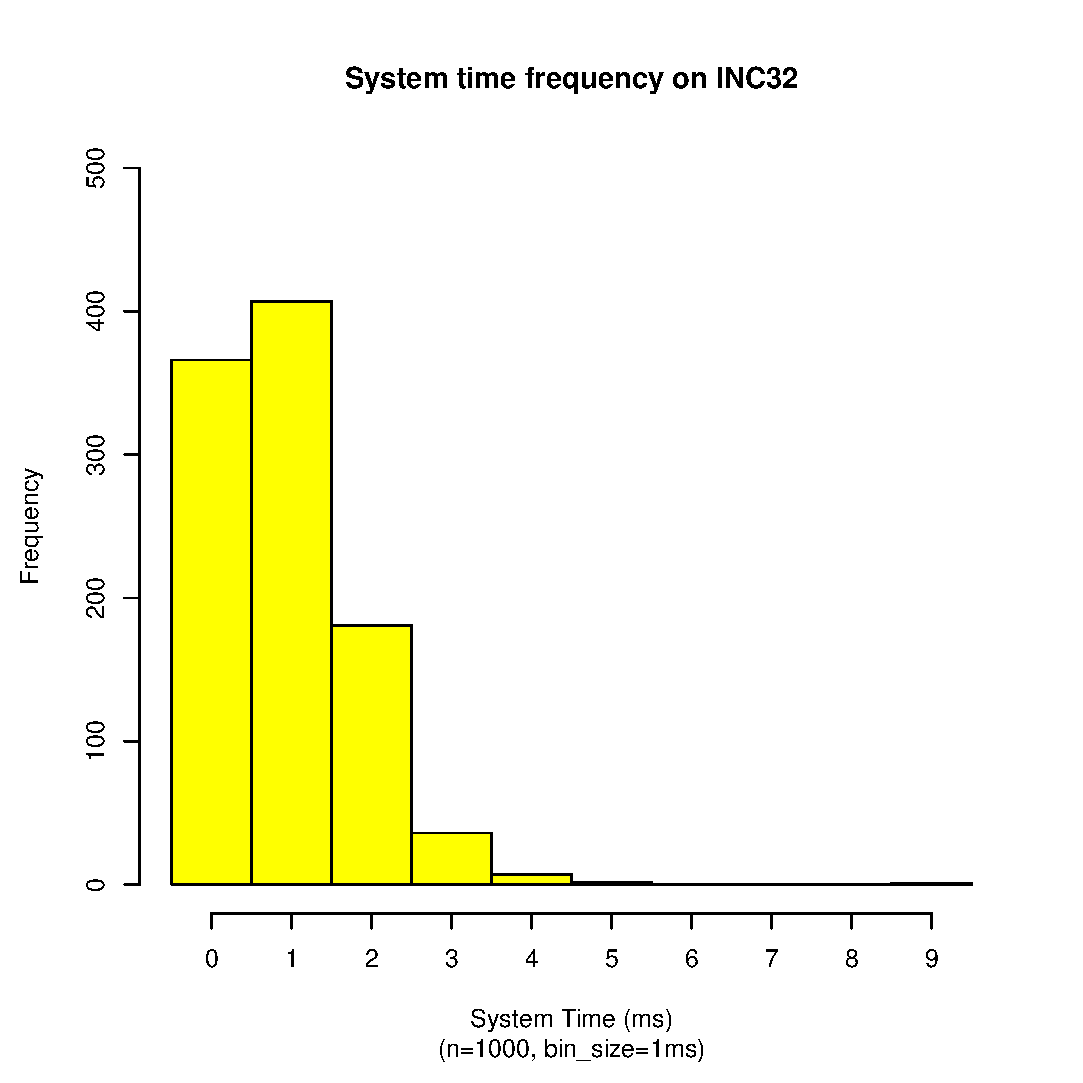
\includegraphics[scale=0.43]{u_s_time/32_sec_st_hist.eps}
		\label{fig:inc32_hist_st}
	}
	\subfigure[System time frequency on INC64]{
		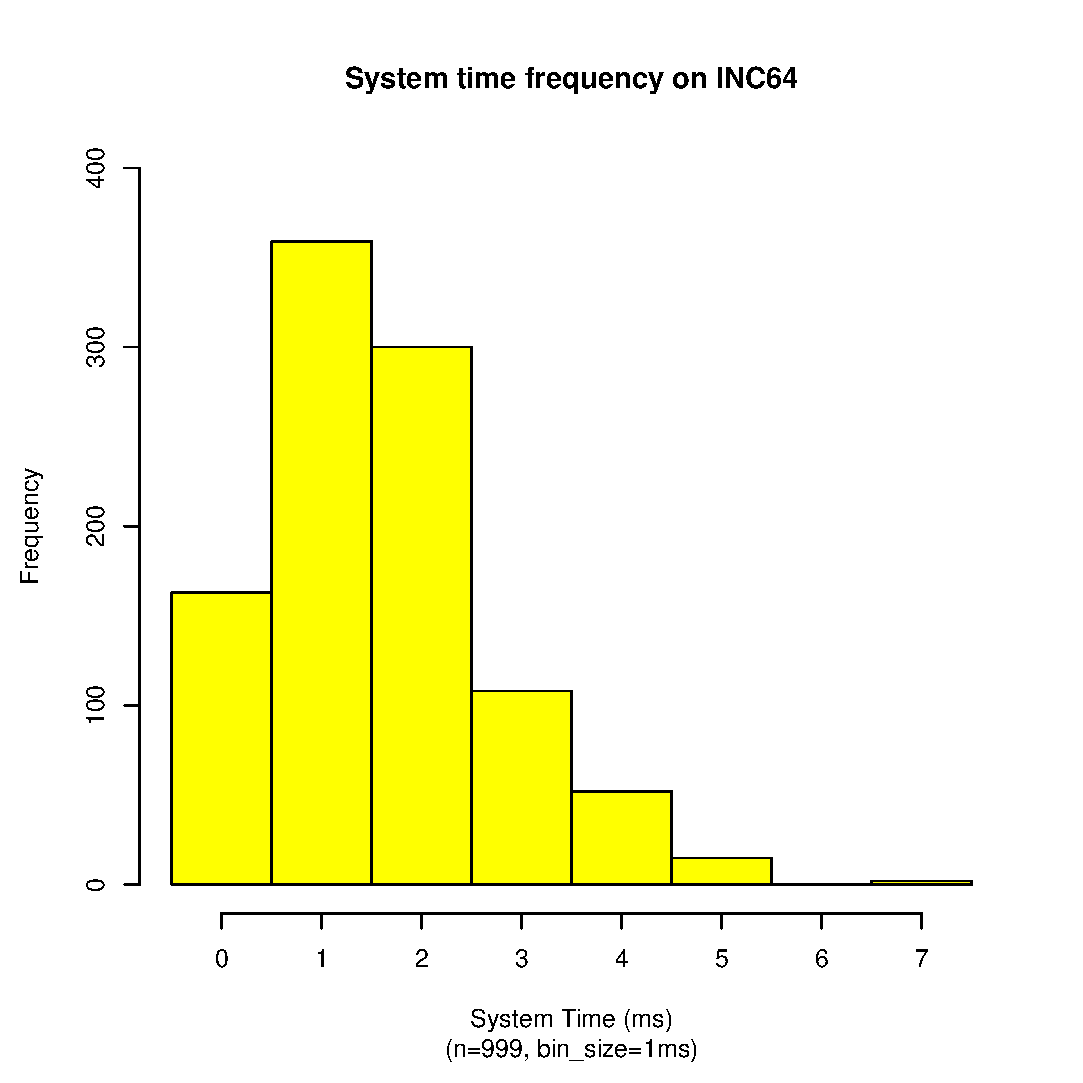
\includegraphics[scale=0.43]{u_s_time/64_sec_st_hist.eps}
		\label{fig:inc64_hist_st}
	}
	\caption{System Time Histograms of INC16 ... INC64\label{fig:st_hist2}}
\end{figure}

\begin{figure}[hp!]
	\centering
	\subfigure[System time frequency on INC128]{
		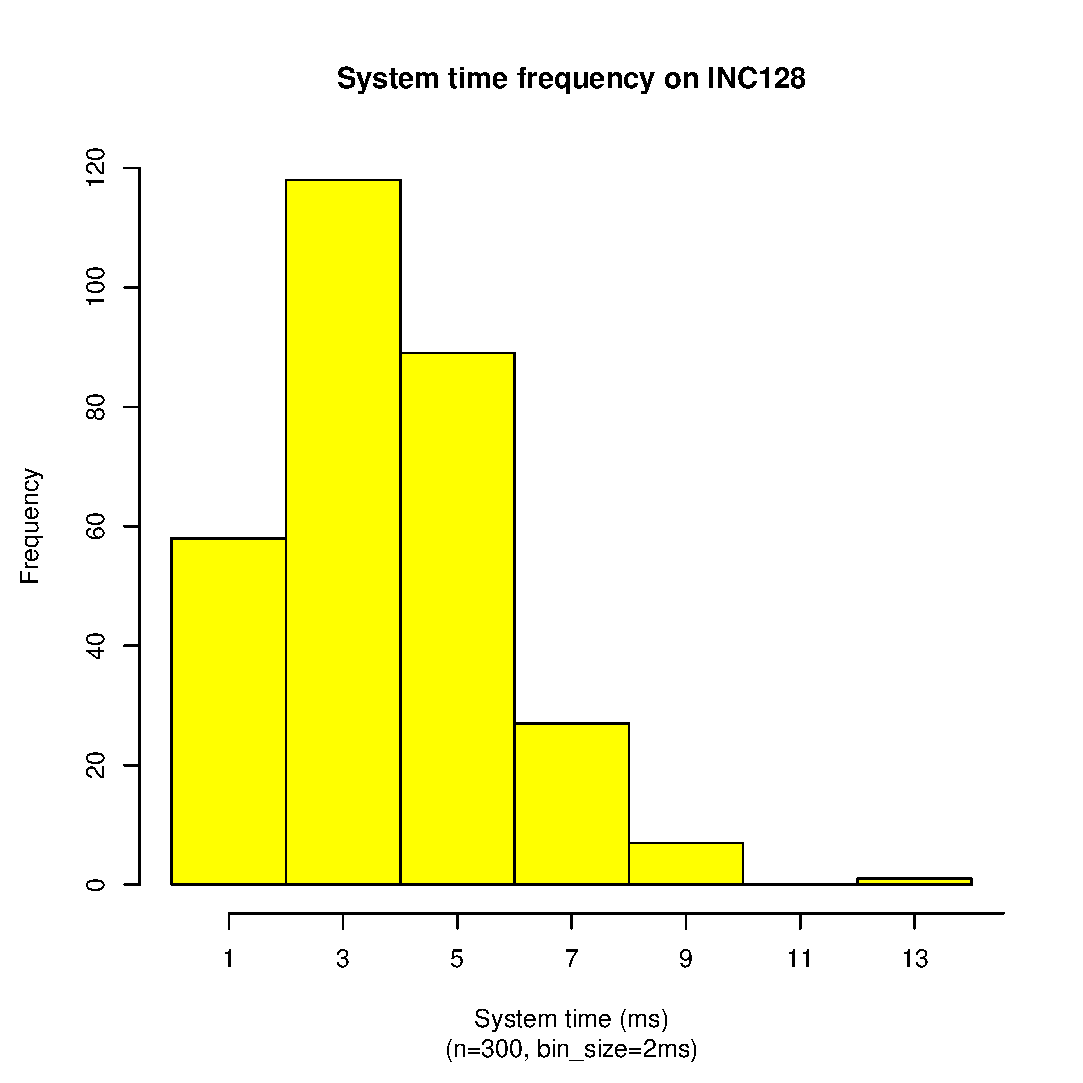
\includegraphics[scale=0.43]{u_s_time/128_sec_st_hist.eps}
		\label{fig:inc128_hist_st}
	}
	\subfigure[System time frequency on INC256]{
		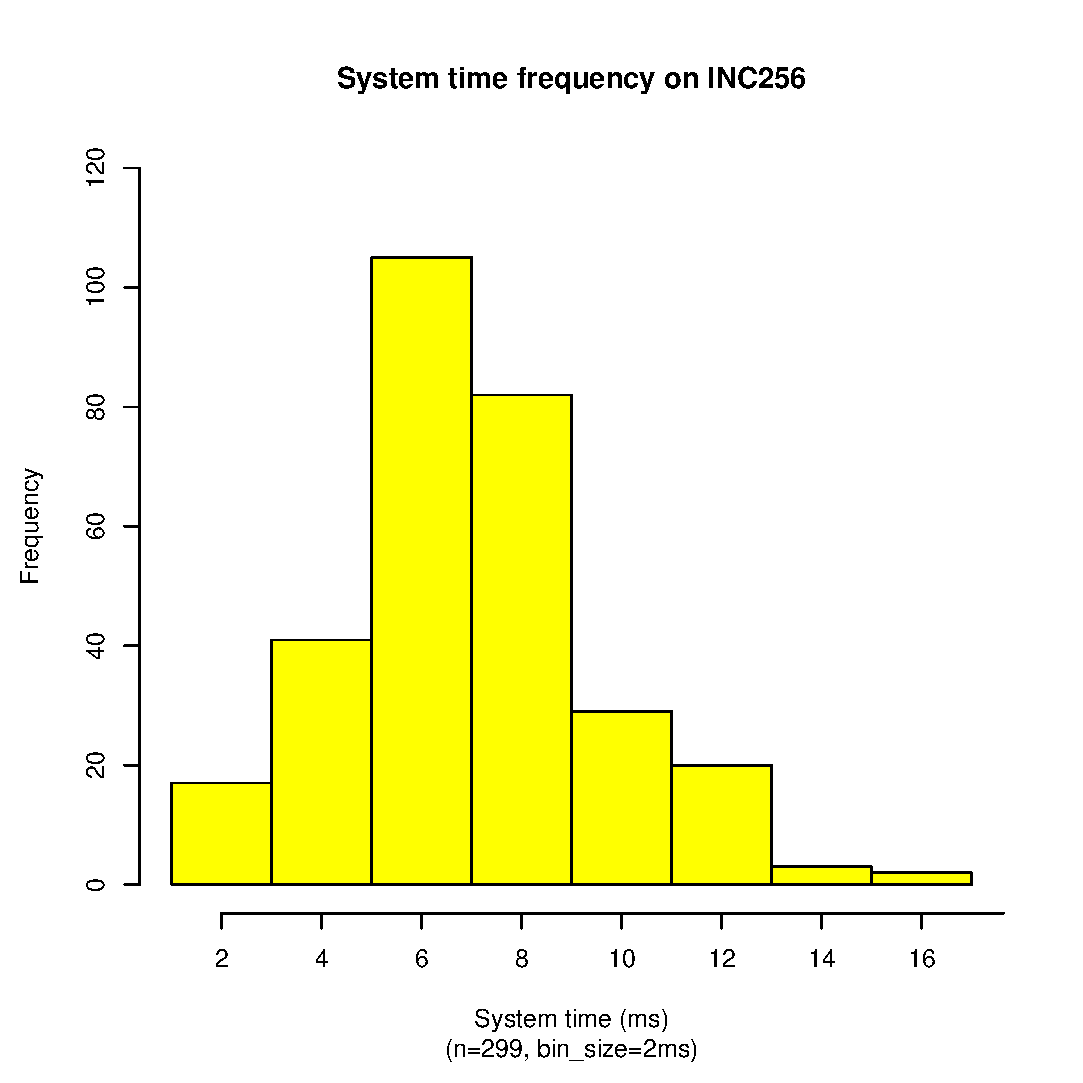
\includegraphics[scale=0.43]{u_s_time/256_sec_st_hist.eps}
		\label{fig:inc256_hist_st}
	}
	\subfigure[System time frequency on INC512]{
		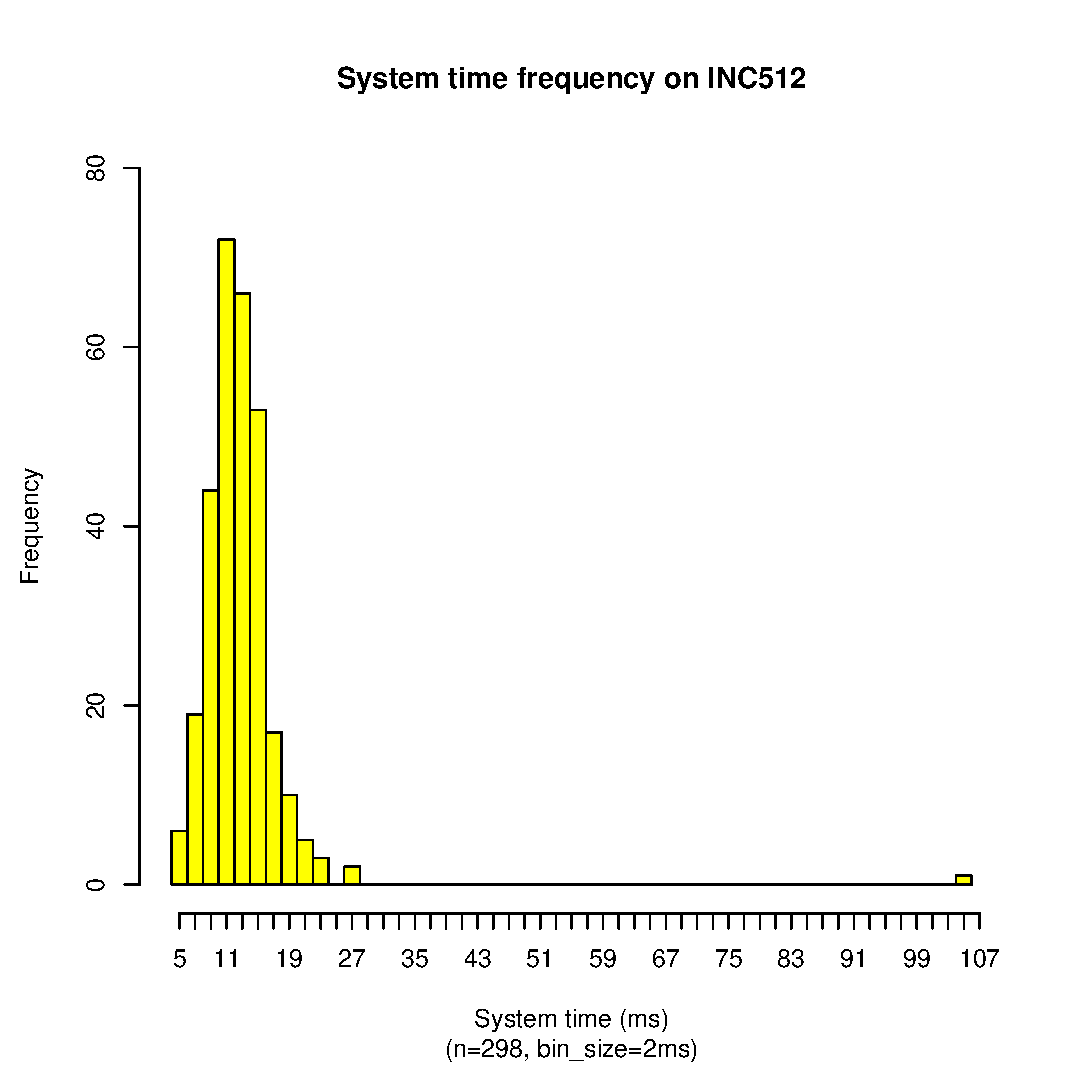
\includegraphics[scale=0.43]{u_s_time/512_sec_st_hist.eps}
		\label{fig:inc512_hist_st}
	}
	\subfigure[System time frequency on INC1024]{
		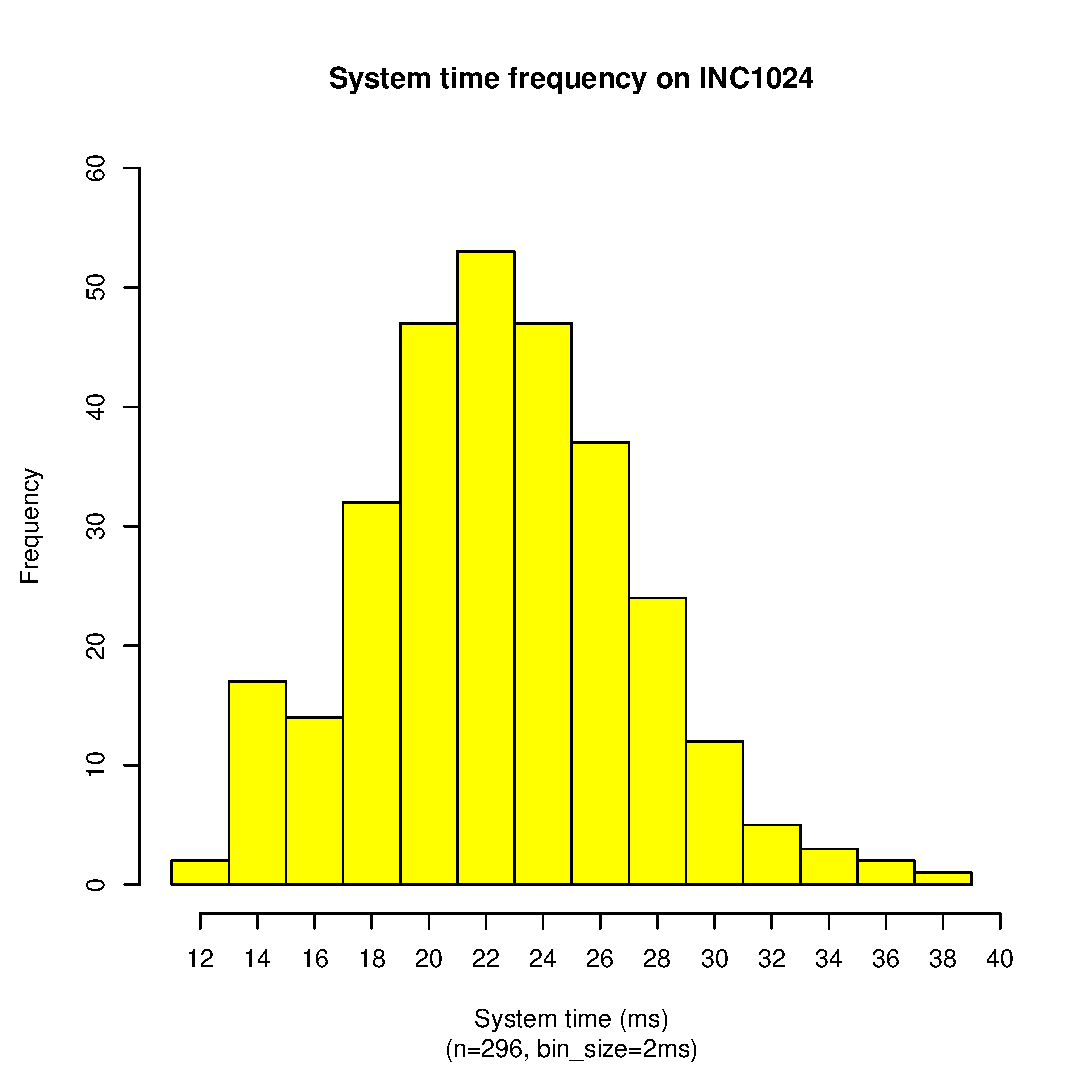
\includegraphics[scale=0.43]{u_s_time/1024_sec_st_hist.eps}
		\label{fig:inc1024_hist_st}
	}
	\caption{System Time Histograms of INC256 ... INC1024~\label{fig:st_hist3}}
\end{figure}

\begin{figure}[t]
	\centering
	\subfigure[System time frequency on INC2048]{
		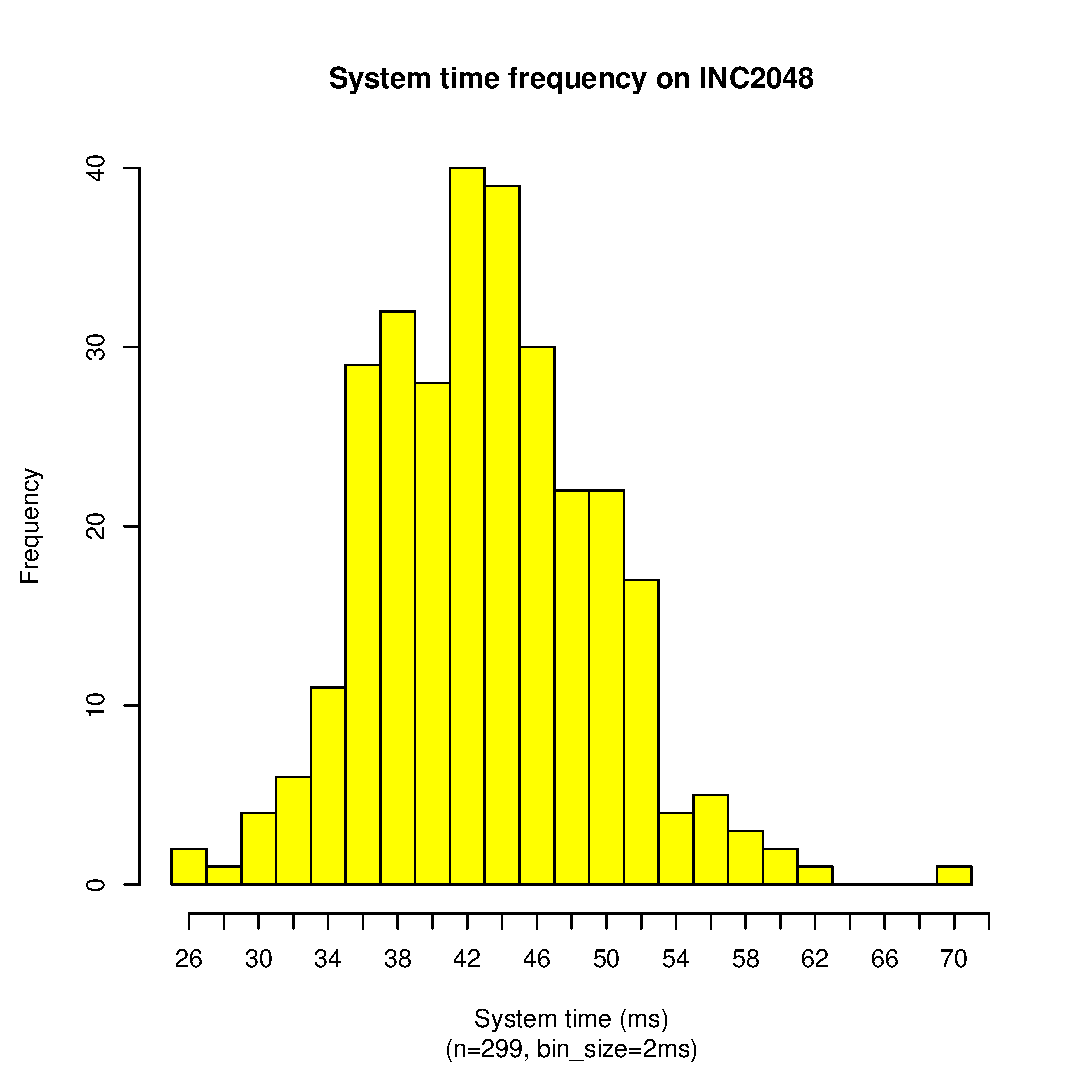
\includegraphics[scale=0.43]{u_s_time/2048_sec_st_hist.eps}
		\label{fig:inc2048_hist_st}
	}
	\subfigure[System time frequency on INC4096]{
		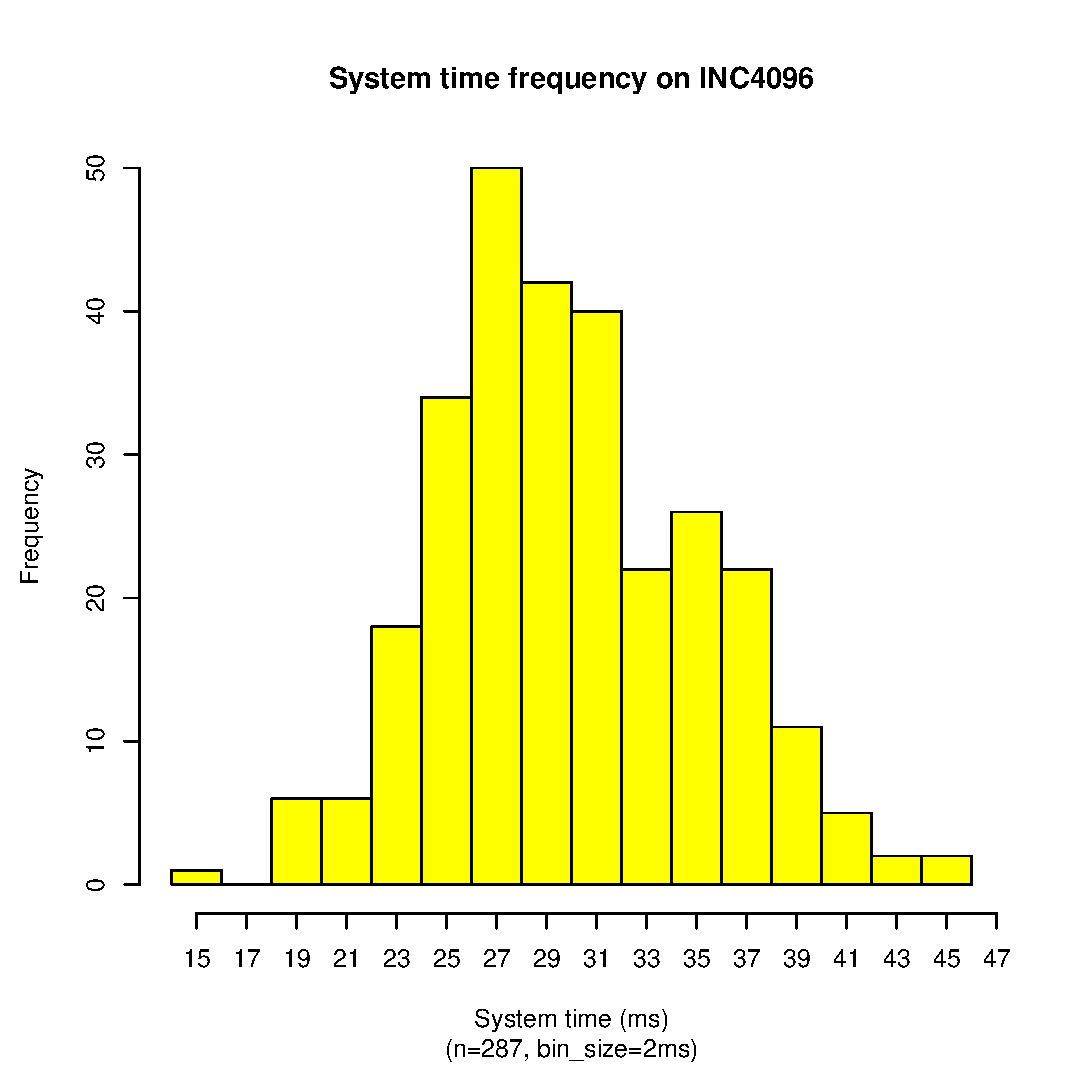
\includegraphics[scale=0.43]{u_s_time/4096_sec_st_hist.eps}
		\label{fig:inc4096_hist_st}
	}
	\caption{System Time Histograms of INC2048 and INC4096~\label{fig:st_hist4}}
\end{figure}

\clearpage
\pagebreak

\subsection{Correlation}

\begin{table}[h]
\begin{center}
\begin{tabular}{|c|c|c|} \hline
 						   & INC2048's u time & INC2048's s time\\ \hline
INC2048's u time  &	 -  &  0.05\\ \hline					
daemon u time & 0.56 & 0.61\\ \hline
daemon s time & 0.48 & 0.57\\ \hline
daemon minor faults &  0.53 & 0.62\\ \hline
daemon major faults & 0.55 & 0.59 \\ \hline
daemon read bytes & 0.55 & 0.59 \\ \hline
daemon read char & 0.56 & 0.61\\ \hline
daemon read sys calls & 0.57 & 0.63\\ \hline
daemon write bytes & 0.57 &  0.64\\ \hline
daemon write char & 0.53 & 0.62\\ \hline
%write sys calls & N/A & N/A\\ \hline
\end{tabular}
\end{center}
\vspace{-.2in}
\caption{Correlation of user and system time of INC2048 with some daemon measures\label{tab:corr_table2}}
\end{table}

\begin{table}[h]
\begin{center}
\begin{tabular}{|c|c|c|} \hline
 						   & INC4096's u time & INC4096's s time\\ \hline
INC4096's u time  &	 -  & -0.30 \\ \hline					
daemon u time & 0.1 & {\bf 0.3} \\ \hline
daemon s time & -0.09 & {\bf 0.19} \\ \hline
daemon minor faults & {\bf 0.11} & {\bf 0.32} \\ \hline
%read bytes & N/A & N/A
daemon read char & 0.1 & {\bf 0.32} \\ \hline
daemon read sys calls & 0.11 & {\bf 0.32} \\ \hline
daemon write bytes & 0 & {\bf 0.26} \\ \hline
daemon write char & 0.11 & {\bf 0.32}\\ \hline
%write sys calls & N/A & N/A
\end{tabular}
\end{center}
\vspace{-.2in}
\caption{Correlation of user and system time of INC4096 with some daemon measures\label{tab:corr_table}}
\end{table}

\clearpage
\newpage

\subsection{Scatter Plots on Some Significant Correlations}
The following scatter plots correspond to the correlations bold in Table~\ref{tab:corr_table}.

\begin{figure}[htp!]
	\centering
	\subfigure[User time vs. Sum of all daemon system time]{
		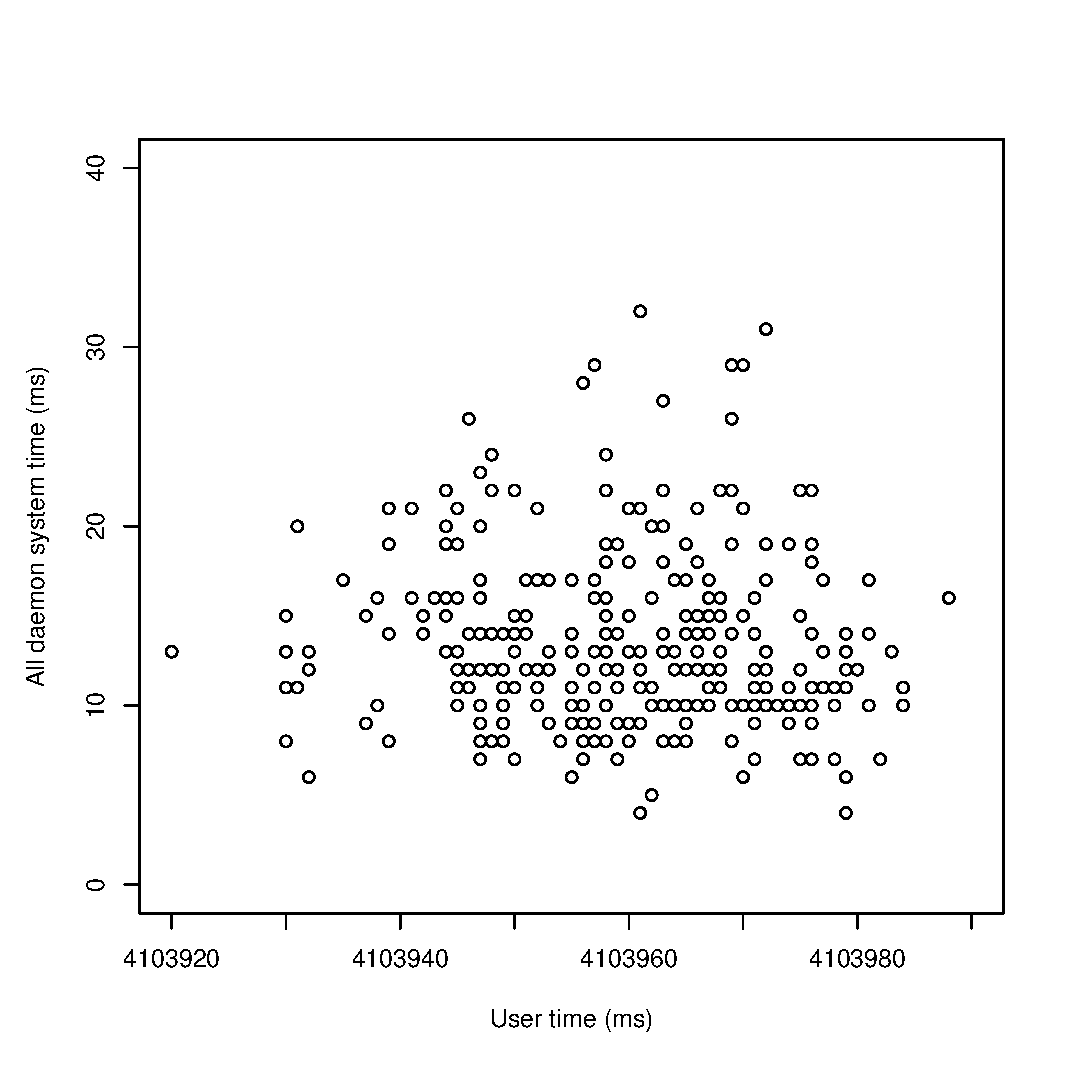
\includegraphics[scale=0.43]{u_s_time/corr_u_as_time.eps}
		\label{fig:corr_u_as_time}
	}
	\subfigure[System time vs. Sum of all  daemon system time]{
		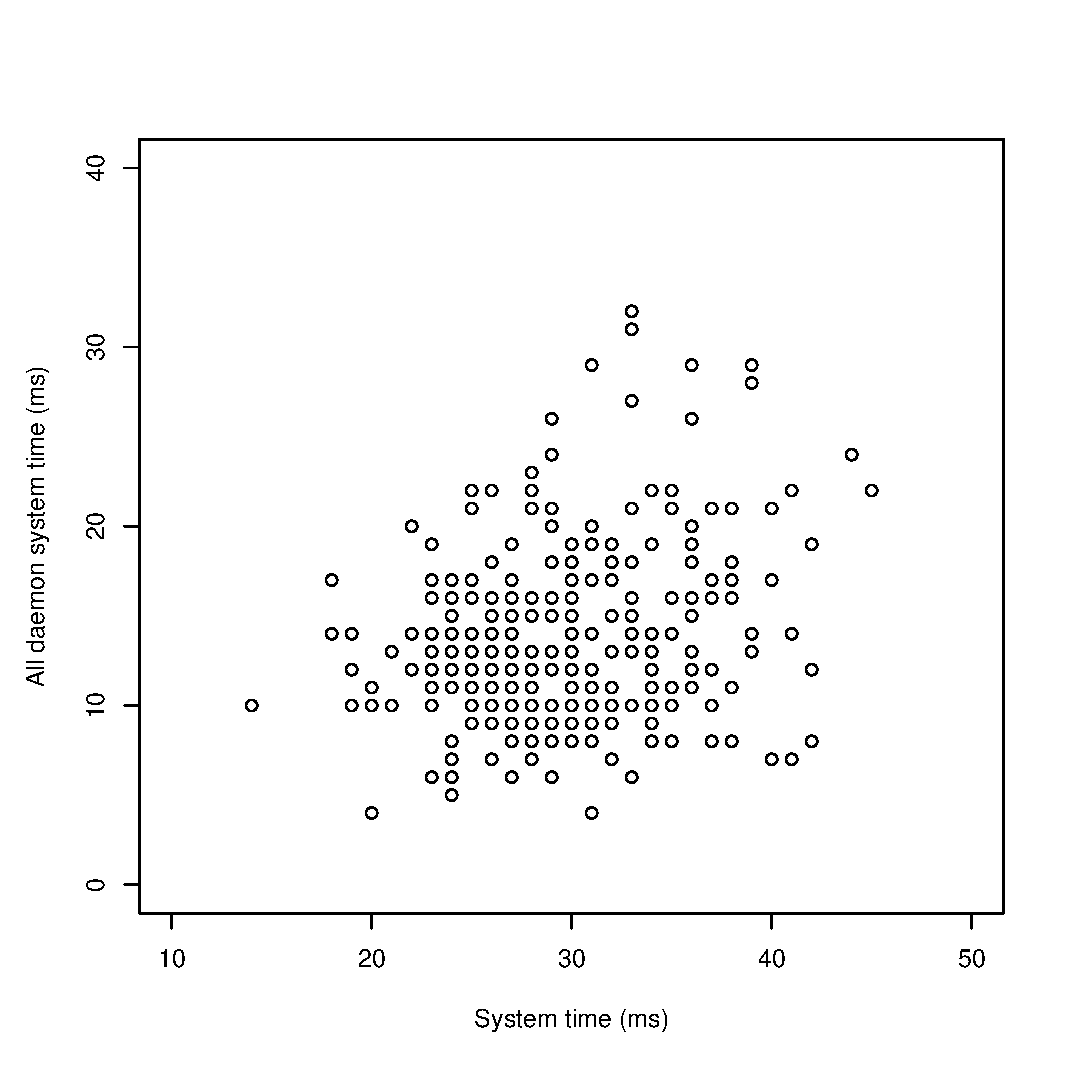
\includegraphics[scale=0.43]{u_s_time/corr_s_as_time.eps}
		\label{fig:corr_s_as_time}
	}
	\subfigure[User time vs. Sum of all  daemon minor faults]{
		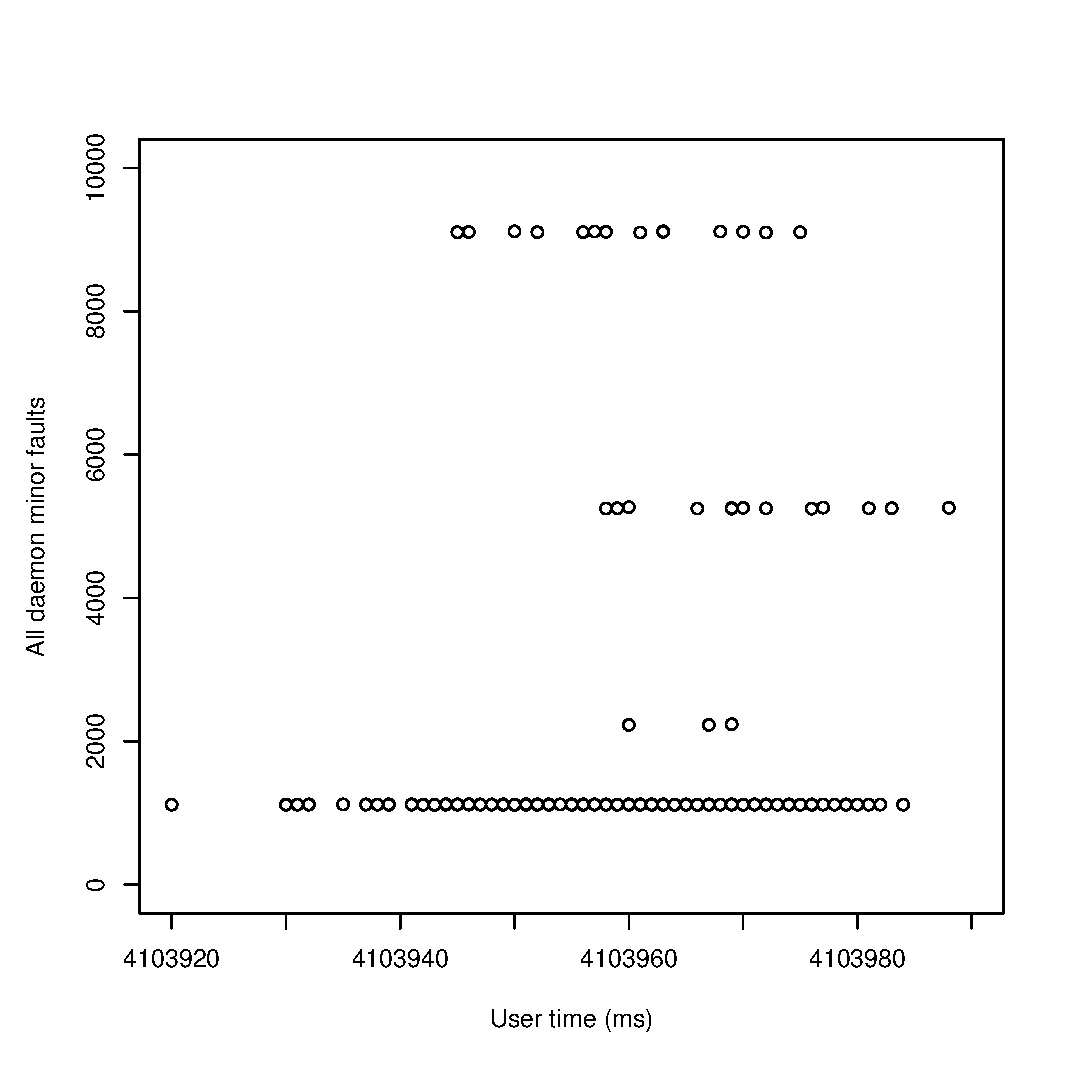
\includegraphics[scale=0.43]{u_s_time/corr_mnf_u_time.eps}
		\label{fig:corr_u_mnf}
	}
	\subfigure[System time vs. Sum of all  daemon minor faults]{
		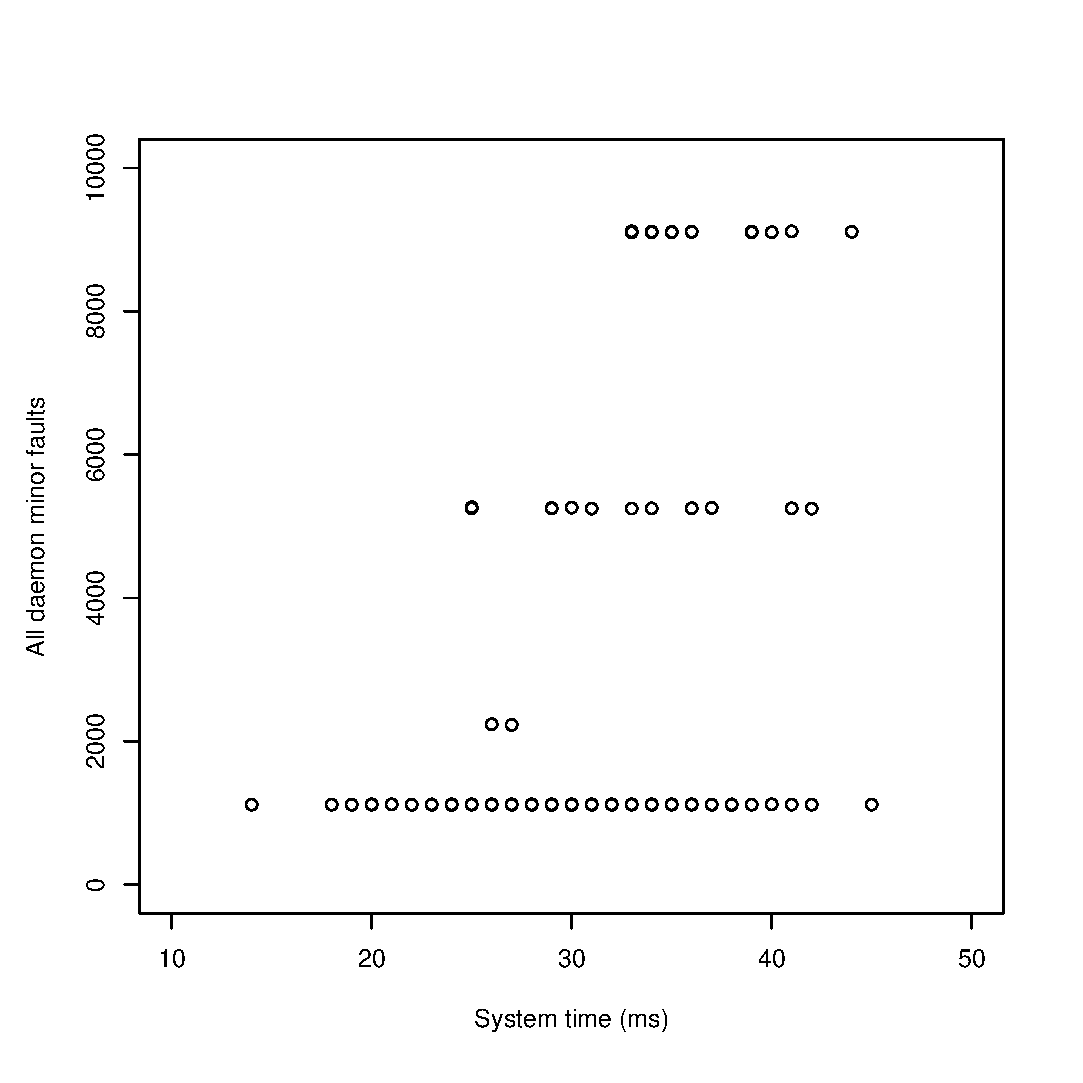
\includegraphics[scale=0.43]{u_s_time/corr_mnf_s_time.eps}
		\label{fig:corr_s_mnf}
	}
	\caption{Scatter plots between measures on INC4096~\label{fig:corr1}}
\end{figure}

\begin{figure}[htp!]
	\centering
	\subfigure[System time vs. Sum of all  daemon read char]{
		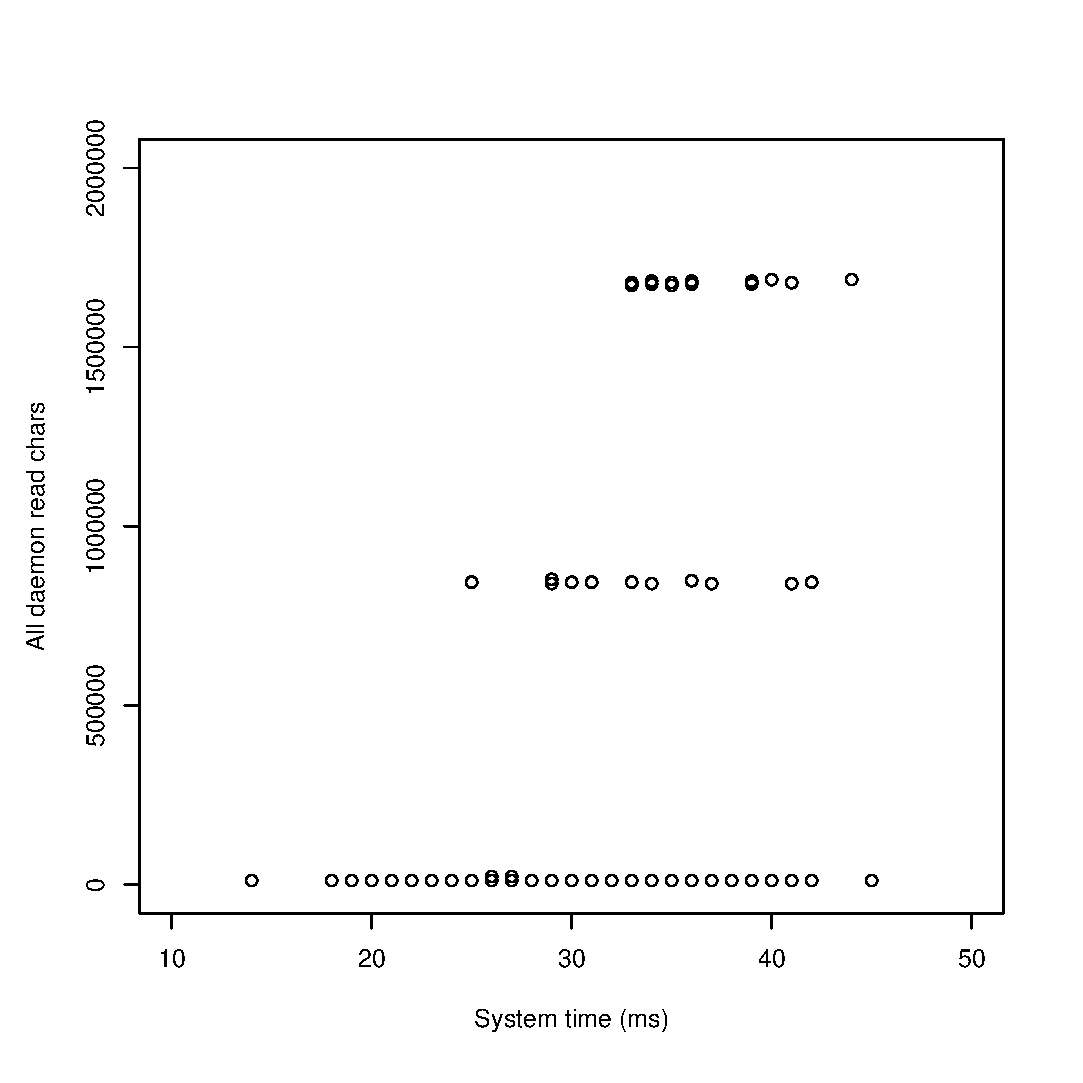
\includegraphics[scale=0.43]{u_s_time/corr_s_rchar.eps}
		\label{fig:corr_s_rchar}
	}
	\subfigure[System time vs. Sum of all  daemon read syscalls]{
		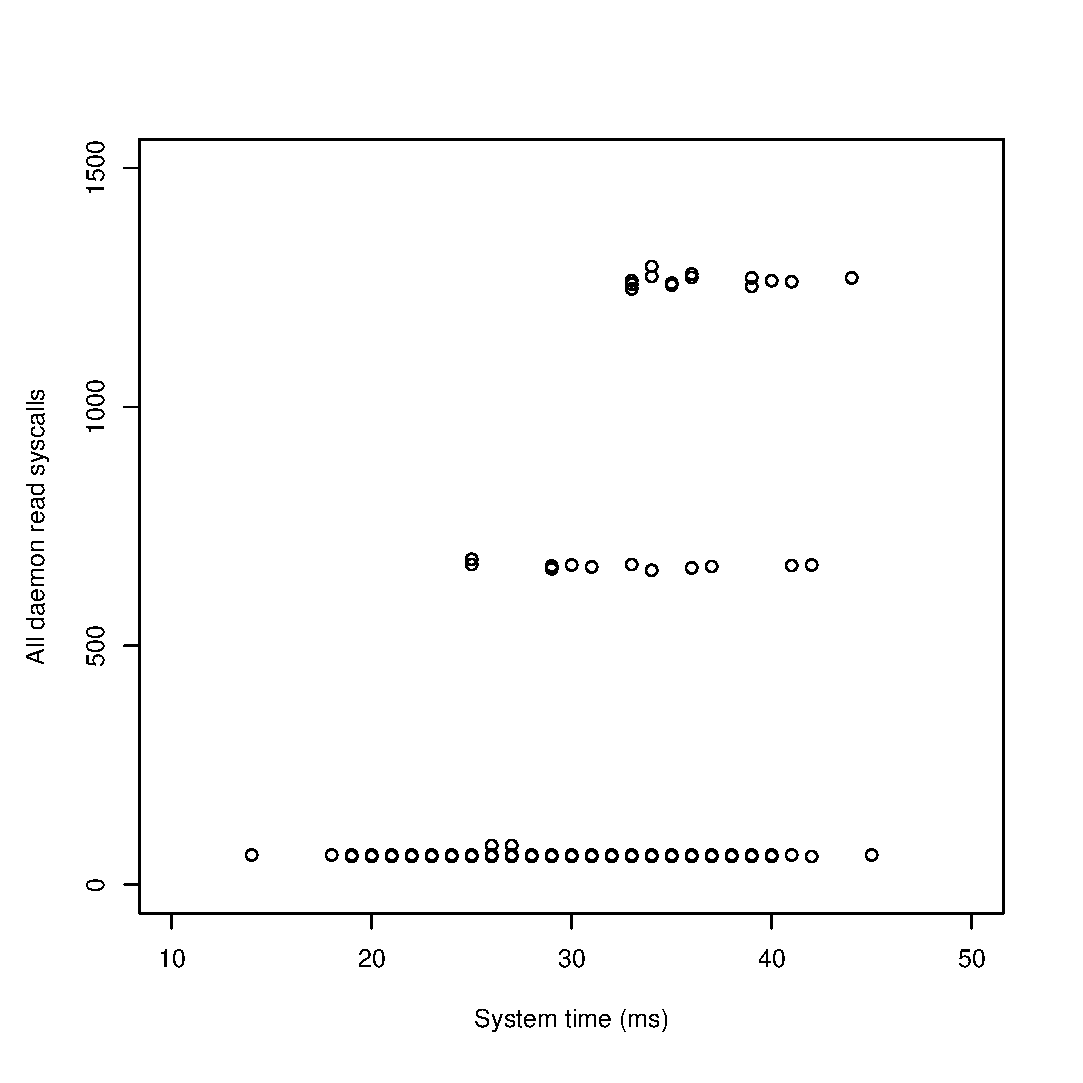
\includegraphics[scale=0.43]{u_s_time/corr_s_rsysc.eps}
		\label{fig:corr_s_rsysc}
	}
	\subfigure[System time vs. Sum of all  daemon write bytes]{
		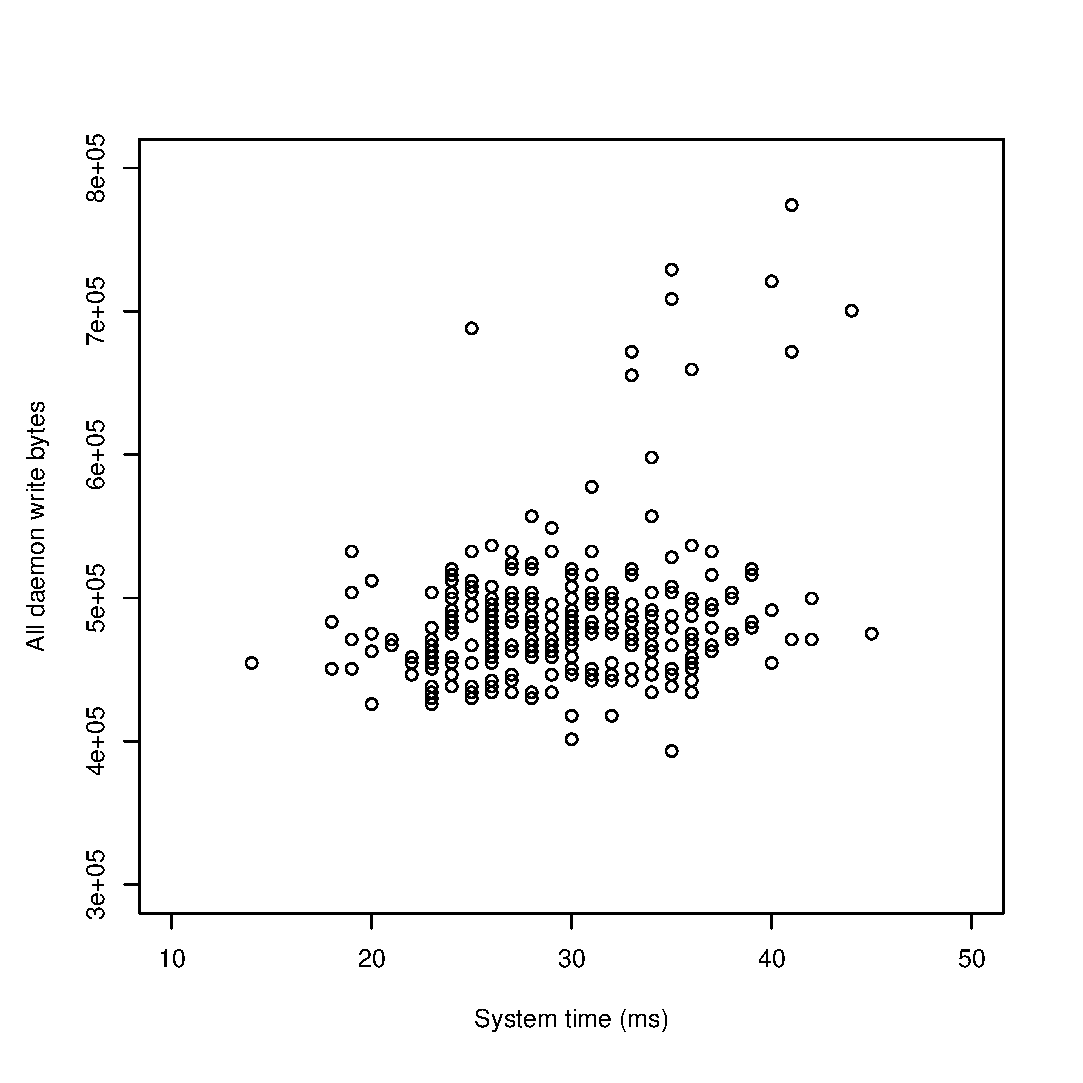
\includegraphics[scale=0.43]{u_s_time/corr_s_wbytes.eps}
		\label{fig:corr_s_wbytes}
	}
	\subfigure[System time vs. Sum of all daemon write char]{
		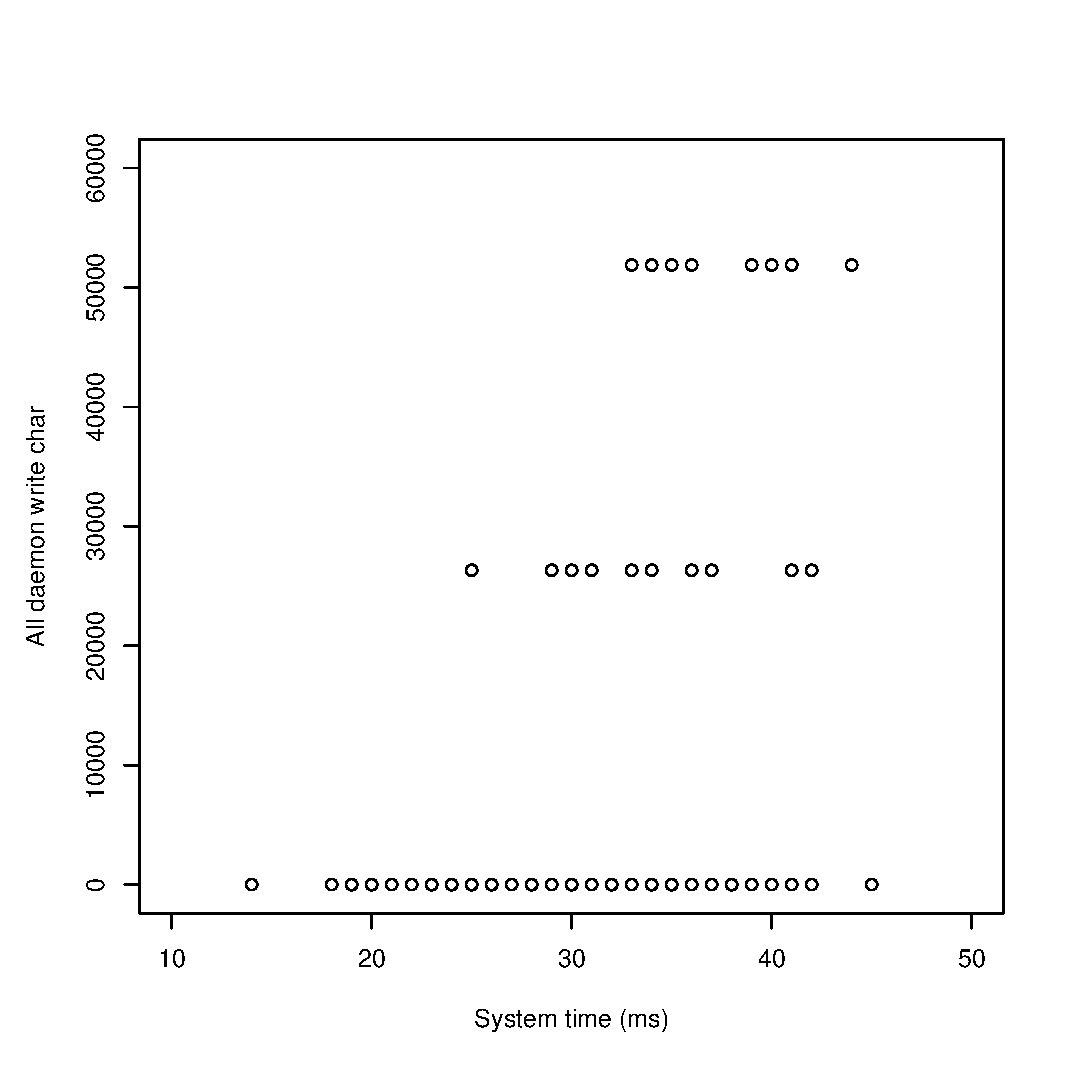
\includegraphics[scale=0.43]{u_s_time/corr_s_wchar.eps}
		\label{fig:corr_s_wchar}
	}
	\caption{Scatter plots between measures on INC4096~\label{fig:corr2}}
\end{figure}

\clearpage

\subsection{Further Investigation of Some Samples}

\subsubsection{Samples in Fig.~\ref{fig:corr_u_mnf}}

\begin{table}[h]
\begin{center}
\begin{tabular}{|c|c|c|c|c|c|c|c|c|c|c|c|} \hline
proc name (id) & u time & s time & min flt & maj flt & r bytes & r char & r sysc & w bytes & w char & w sysc\\ \hline
INC4096 (3559) & 4103920 & 36 & 0 & 0 & 0 & 1 & 1 & 0 & 0 & 0 \\ \hline
proc\_monitor (25917) & 194 & 6 & 2 & 0 & 0 & 0 & 0 & 0 & 0 & 0 \\ \hline
md0\_raid1 (484) & 0 &  3 & 0 & 0 & 0 & 0 & 0 & 0 & 0 & 0 \\ \hline
java (3549) & 2 & 1 & 1093 & 0 & 0 & 11480 & 20 & 0 & 0 & 0 \\ \hline
cifsd (1927) & 0 & 1 & 0 & 0 & 0 & 0 & 0 & 0 & 0 & 0 \\ \hline
kblockd/0 (16) & 0 & 1 & 0 & 0 & 0 & 0 & 0 & 0 & 0 & 0 \\ \hline
ntpd (28232) & 0 & 1 & 1 & 0 & 0 & 0 & 42 & 4096 & 7 & 0 \\ \hline
\end{tabular}
\end{center}
\caption{Observed values of measures of processes on the leftmost sample in Fig.~\ref{fig:corr_u_mnf}~\label{tab:breakdown}}
\end{table}

\begin{table}[h]
\begin{center}
\begin{tabular}{|c|c|c|c|c|c|c|c|c|c|c|c|} \hline
proc name (id) & u time & s time & min flt & maj flt & r bytes & r char & r sysc & w bytes & w char & w sysc\\ \hline
INC4096 (3559) & 4103984 & 19 & 0 & 0 & 0 & 1 & 1 & 0 & 0 & 0 \\ \hline
proc\_monitor (25917) & 190 & 6 & 2 & 0 & 0 & 0 & 0 & 0 & 0 & 0 \\ \hline
java (3549) & 2 & 1 & 1093 & 0 & 0 & 11480 & 20 & 0 & 0 & 0 \\ \hline
md0\_raid1 (484) & 0 & 3 & 0 & 0 & 0 & 0 & 0 & 0 & 0 & 0 \\ \hline
ntpd (28232) & 0 & 0 & 1 & 0 & 0 & 0 & 39 & 4096 & 7 & 0 \\ \hline
java (4108) & 0 & 0  & 20 & 0 & 0 & 0 & 0 & 0 & 0 & 0 \\ \hline
\end{tabular}
\end{center}
\caption{Observed values of measures of processes on the second rightmost sample in Fig.~\ref{fig:corr_u_mnf}~\label{tab:breakdown2}}
\end{table}

\begin{table}[h]
\begin{center}
\begin{tabular}{|c|c|c|c|c|c|c|c|c|c|c|c|} \hline
proc name (id) & u time & s time & min flt & maj flt & r bytes & r char & r sysc & w bytes & w char & w sysc\\ \hline
INC4096 (3559) & 4103988 & 25 & 0 & 0 & 0 & 1 & 1 & 0 & 0 & 0 \\ \hline
proc\_monitor  (25917)  & 194 & 2 & 2 & 0 & 0 & 0 & 0 & 0 & 0 & 0 \\ \hline
sshd (3609) & 8 & 4 & 1382 & 0 & 0 & 512357 & 400 & 0 & 20881 & 0 \\ \hline
bash (3611)  & 4 & 1 & 835 & 0 & 0 & 283911 & 155 & 0 & 136 & 0 \\ \hline
md0\_raid1 (484) & 0 & 3 & 0 & 0 & 0 & 0 & 0 & 0 & 0 & 0 \\ \hline
java (3549) & 2 & 1 & 1093 & 0 & 0 & 11480 & 20 & 0 & 0 & 0 \\ \hline
cifsd (1927) & 0 & 2 & 0 & 0 & 0 & 0 & 0 & 0 & 0 & 0 \\ \hline
java (3606) & 0 & 1 & 22 & 0 & 0 & 0 & 0 & 0 & 0 & 0 \\ \hline
jbd2/md0-8 (497) & 0 & 1 & 0 & 0 & 0 & 0 & 0 & 450560 & 0 & 0 \\ \hline
kblockd/0 (16) & 0 & 1 & 0 & 0 & 0 & 0 & 0 & 0 & 0 & 0 \\ \hline
grep (3617) & 1 & 0 & 311 & 0 & 0 & 5417 & 11 & 0 & 0 & 0 \\ \hline
bash (3612) & 0 & 0 & 158 & 0 & 0 & 0 & 0 & 0 & 0 & 0 \\ \hline
consoletype (3613) & 0 & 0 & 127 & 0 & 0 & 1956 & 6 & 0 & 7 & 0 \\ \hline
bash (3614) & 0 & 0 & 174 & 0 & 0 & 0 & 0 & 0 & 0 & 0 \\ \hline
uname (3615) & 0 & 0 & 189 & 0 & 0 & 1956  & 6 & 0 & 7 & 0 \\ \hline
sshd (3610) & 0 & 0 & 425 & 0 & 0 & 22656 & 29 & 0 & 4630 & 0 \\ \hline
sshd (2105) & 0 & 0 & 14 & 0 & 0 & 0 & 0 & 0 & 594 & 0 \\ \hline
bash (3618) & 0 & 0 & 170 & 0 & 0 & 0 & 0 & 0 & 0 & 0 \\ \hline
id (3619) & 0 & 0 & 225 & 0 & 0 & 4352 & 12 & 0 & 2 & 0 \\ \hline
ntpd (28232) & 0 & 0 & 1 & 0 & 0 & 0 & 42 & 4096 & 7 & 0 \\ \hline
bash (3616) & 0 & 0 & 131 & 0 & 0 & 0 & 0 & 0 & 61 & 0 \\ \hline
\end{tabular}
\end{center}
\caption{Observed values of measures of processes on the rightmost sample in Fig.~\ref{fig:corr_u_mnf}~\label{tab:breakdown1}}
\end{table}

\clearpage
\newpage

\subsubsection{Samples in Fig.~\ref{fig:corr_s_wbytes}}

\begin{table}[h]
\begin{center}
\begin{tabular}{|c|c|c|c|c|c|c|c|c|c|c|c|} \hline
proc name (id) & u time & s time & min flt & maj flt & r bytes & r char & r sysc & w bytes & w char & w sysc\\ \hline
INC4096 (3559) & 4103981 & 14 & 0 & 0 & 0 & 1 & 1 & 0 & 0 & 0 \\ \hline
proc\_monitor (25917) & 194 & 2 & 2 & 0 & 0 & 0 & 0 & 0 & 0 & 0 \\ \hline
md0\_raid1 (484) & 0 & 5 & 0 & 0 & 0 & 0 & 0 & 0 & 0 & 0 \\ \hline
java (3549) & 2 & 1 & 1093 & 0 & 0 & 11480 & 20 & 0 & 0 & 0 \\ \hline
flush-9:0 (3548) & 0 & 2 & 0 & 0 & 0 & 0 & 0 & 0 & 0 & 0 \\ \hline
ntpd (28232) & 0 & 0 & 1 & 0 & 0 & 0 & 42 & 4096 & 7 & 0 \\ \hline
java (4585) & 0 & 0 & 20 & 0 & 0 & 0 & 0 & 0 & 0 & 0 \\ \hline
\end{tabular}
\end{center}
\caption{Observed values of measures of processes on the leftmost sample in Fig.~\ref{fig:corr_s_wbytes}~\label{tab:breakdown4}}
\end{table}

\begin{table}[h]
\begin{center}
\begin{tabular}{|c|c|c|c|c|c|c|c|c|c|c|c|} \hline
proc name (id) & u time & s time & min flt & maj flt & r bytes & r char & r sysc & w bytes & w char & w sysc\\ \hline
INC4096 (3559) & 4103958 & 44 & 0 & 0 & 0 & 1 & 1 & 0 & 0 & 0 \\ \hline
proc\_monitor (25917) & 194 & 2 & 2 & 0 & 0 & 0 & 0 & 0 & 0 & 0 \\ \hline
sshd (4877) & 10 & 4 & 1382 & 0 & 0 & 519568 & 392 & 0 & 20868 & 0 \\ \hline
sshd (4886) & 10 & 3 & 1383 & 0 & 0 & 515456 & 393 & 0 & 20868 & 0 \\ \hline
grep (4888) & 6 & 1 & 994 & 0 & 0 & 287034 & 154 & 0 & 136 & 0 \\ \hline
grep (4879) & 3 & 2 & 991 & 0 & 0 & 286801 & 159 & 0 & 136 & 0 \\ \hline
java (3549) & 2 & 1 & 1093 & 0 & 0 & 11480 & 20 & 0 & 0 & 0 \\ \hline
md0\_raid1 (484) & 0 & 3 & 0 & 0 & 0 & 0 & 0 & 0 & 0 & 0 \\ \hline
sshd (4878) & 2 & 1 & 424 & 0 & 0 & 22403 & 26 & 0 & 4268 & 0 \\ \hline
jbd2/md0-8 (497) & 0 & 2 & 0 & 0 & 0 & 0 & 0 & 696320 & 0 & 0 \\ \hline
flush-9:0 (3548) & 0 & 2 & 0 & 0 & 0 & 0 & 0 & 0 & 0 & 0 \\ \hline
cifsd (1927) & 0 & 1 & 0 & 0 & 0 & 0 & 0 & 0 & 0 & 0 \\ \hline
kblockd/0 (16) & 0 & 1 & 0 & 0 & 0 & 0 & 0 & 0 & 0 & 0 \\ \hline
grep (4892) & 0 & 1 & 309 & 0 & 0 & 5417 & 11 & 0 & 0 & 0 \\ \hline
grep (4883) & 1 & 0 & 310 & 0 & 0 & 5417 & 11 & 0 & 0 & 0 \\ \hline
id (4894) & 0 & 0 & 226 & 0 & 0 & 4352 & 12 & 0 & 2 & 0 \\ \hline
bash (4884) & 0 & 0 & 164 & 0 & 0 & 0 & 0 & 0 & 0 & 0 \\ \hline
id (4885) & 0 & 0 & 226 & 0 & 0 & 0 & 12 & 0 & 2 & 0 \\ \hline
sshd (2105) & 0 & 0 & 28 & 0 & 0 & 0 & 0 & 0 & 1188 & 0 \\ \hline
sshd (4887) & 0 & 0 & 425 & 0 & 0 & 22403 &26 & 0 & 4268 & 0 \\ \hline
ntpd (20232) & 0 & 0 & 1 & 0 & 0 & 0 & 42 & 4096 & 7 & 0 \\ \hline
bash (4880) & 0 & 0 & 165 & 0 & 0 & 0 & 0 & 0 & 0 & 0 \\ \hline
uname (4890)  & 0 & 0 & 190 & 0 & 0 & 1956  & 6 & 0 & 7 & 0 \\ \hline
bash (4891) & 0 & 0 & 128 & 0 & 0 & 0 & 0 & 0 & 61 & 0 \\ \hline
java  (4874) & 0 & 0 & 20 & 0 & 0 & 0 & 0 & 0 & 0 & 0 \\ \hline
bash (4893) & 0 & 0 & 164 & 0 & 0 & 0 & 0 & 0 & 0 & 0 \\ \hline
uname (4881)  & 0 & 0 & 191 & 0 & 0 & 1956  & 6 & 0 & 7 & 0 \\ \hline
bash (4889) & 0 & 0 & 165 & 0 & 0 & 0 & 0 & 0 & 0 & 0 \\ \hline
\end{tabular}
\end{center}
\caption{Observed values of measures of processes on the second rightmost sample in Fig.~\ref{fig:corr_s_wbytes}~\label{tab:breakdown5}}
\end{table}

\begin{table}[h]
\begin{center}
\begin{tabular}{|c|c|c|c|c|c|c|c|c|c|c|c|} \hline
proc name (id) & u time & s time & min flt & maj flt & r bytes & r char & r sysc & w bytes & w char & w sysc\\ \hline
INC4096 (3559) & 4103948 & 45 & 0 & 0 & 0 & 1 & 1 & 0 & 0 & 0 \\ \hline
proc\_monitor (25917) & 190 & 10 & 2 & 0 & 0 & 0 & 0 & 0 & 0 & 0 \\ \hline
md0\_raid1 (484) & 0 & 5 & 0 & 0 & 0 & 0 & 0 & 0 & 0 & 0 \\ \hline
jbd2/md0-8 (497) & 0 & 3 & 0 & 0 & 0 & 0 & 0 & 471040 & 0 & 0 \\ \hline
java (3549) & 2 & 1 & 1093 & 0 & 0 & 11480 & 20 & 0 & 0 & 0 \\ \hline
cifsd (1927) & 0 & 2 & 0 & 0 & 0 & 0 & 0 & 0 & 0 & 0 \\ \hline
flush-9:0 (3548) & 0 & 1 & 0 & 0 & 0 & 0 & 0 & 0 & 0 & 0 \\ \hline
java (5022) & 1 & 0 & 21 & 0 & 0 & 0 & 0 & 0 & 0 & 0 \\ \hline
ntpd (28232) & 0 & 0 & 1 & 0 & 0 & 0 & 42 & 4096 & 7 & 0 \\ \hline
\end{tabular}
\end{center}
\caption{Observed values of measures of processes on the rightmost sample in Fig.~\ref{fig:corr_s_wbytes}~\label{tab:breakdown6}}
\end{table}
